\documentclass[twoside]{book}

% Packages required by doxygen
\usepackage{calc}
\usepackage{doxygen}
\usepackage{graphicx}
\usepackage[utf8]{inputenc}
\usepackage{makeidx}
\usepackage{multicol}
\usepackage{multirow}
\usepackage{textcomp}
\usepackage[table]{xcolor}

% Font selection
\usepackage[T1]{fontenc}
\usepackage{mathptmx}
\usepackage[scaled=.90]{helvet}
\usepackage{courier}
\usepackage{amssymb}
\usepackage{sectsty}
\renewcommand{\familydefault}{\sfdefault}
\allsectionsfont{%
  \fontseries{bc}\selectfont%
  \color{darkgray}%
}
\renewcommand{\DoxyLabelFont}{%
  \fontseries{bc}\selectfont%
  \color{darkgray}%
}

% Page & text layout
\usepackage{geometry}
\geometry{%
  a4paper,%
  top=2.5cm,%
  bottom=2.5cm,%
  left=2.5cm,%
  right=2.5cm%
}
\tolerance=750
\hfuzz=15pt
\hbadness=750
\setlength{\emergencystretch}{15pt}
\setlength{\parindent}{0cm}
\setlength{\parskip}{0.2cm}
\makeatletter
\renewcommand{\paragraph}{%
  \@startsection{paragraph}{4}{0ex}{-1.0ex}{1.0ex}{%
    \normalfont\normalsize\bfseries\SS@parafont%
  }%
}
\renewcommand{\subparagraph}{%
  \@startsection{subparagraph}{5}{0ex}{-1.0ex}{1.0ex}{%
    \normalfont\normalsize\bfseries\SS@subparafont%
  }%
}
\makeatother

% Headers & footers
\usepackage{fancyhdr}
\pagestyle{fancyplain}
\fancyhead[LE]{\fancyplain{}{\bfseries\thepage}}
\fancyhead[CE]{\fancyplain{}{}}
\fancyhead[RE]{\fancyplain{}{\bfseries\leftmark}}
\fancyhead[LO]{\fancyplain{}{\bfseries\rightmark}}
\fancyhead[CO]{\fancyplain{}{}}
\fancyhead[RO]{\fancyplain{}{\bfseries\thepage}}
\fancyfoot[LE]{\fancyplain{}{}}
\fancyfoot[CE]{\fancyplain{}{}}
\fancyfoot[RE]{\fancyplain{}{\bfseries\scriptsize Generated on Thu Oct 30 2014 15\-:04\-:36 for digiholo2\-D by Doxygen }}
\fancyfoot[LO]{\fancyplain{}{\bfseries\scriptsize Generated on Thu Oct 30 2014 15\-:04\-:36 for digiholo2\-D by Doxygen }}
\fancyfoot[CO]{\fancyplain{}{}}
\fancyfoot[RO]{\fancyplain{}{}}
\renewcommand{\footrulewidth}{0.4pt}
\renewcommand{\chaptermark}[1]{%
  \markboth{#1}{}%
}
\renewcommand{\sectionmark}[1]{%
  \markright{\thesection\ #1}%
}

% Indices & bibliography
\usepackage{natbib}
\usepackage[titles]{tocloft}
\setcounter{tocdepth}{3}
\setcounter{secnumdepth}{5}
\makeindex

% Hyperlinks (required, but should be loaded last)
\usepackage{ifpdf}
\ifpdf
  \usepackage[pdftex,pagebackref=true]{hyperref}
\else
  \usepackage[ps2pdf,pagebackref=true]{hyperref}
\fi
\hypersetup{%
  colorlinks=true,%
  linkcolor=blue,%
  citecolor=blue,%
  unicode%
}

% Custom commands
\newcommand{\clearemptydoublepage}{%
  \newpage{\pagestyle{empty}\cleardoublepage}%
}


%===== C O N T E N T S =====

\begin{document}

% Titlepage & ToC
\hypersetup{pageanchor=false}
\pagenumbering{roman}
\begin{titlepage}
\vspace*{7cm}
\begin{center}%
{\Large digiholo2\-D }\\
\vspace*{1cm}
{\large Generated by Doxygen 1.8.6}\\
\vspace*{0.5cm}
{\small Thu Oct 30 2014 15:04:36}\\
\end{center}
\end{titlepage}
\clearemptydoublepage
\tableofcontents
\clearemptydoublepage
\pagenumbering{arabic}
\hypersetup{pageanchor=true}

%--- Begin generated contents ---
\chapter{Hierarchical Index}
\section{Class Hierarchy}
This inheritance list is sorted roughly, but not completely, alphabetically\-:\begin{DoxyCompactList}
\item \contentsline{section}{abstract\-\_\-fringe\-\_\-analyser}{\pageref{classabstract__fringe__analyser}}{}
\begin{DoxyCompactList}
\item \contentsline{section}{Takeda\-\_\-\-F\-F\-T\-W\-\_\-fringe\-\_\-analyser}{\pageref{class_takeda___f_f_t_w__fringe__analyser}}{}
\end{DoxyCompactList}
\item \contentsline{section}{abstract\-\_\-smart\-\_\-tile\-\_\-unwrapper}{\pageref{classabstract__smart__tile__unwrapper}}{}
\item \contentsline{section}{abstract\-\_\-smart\-\_\-unwrapper}{\pageref{classabstract__smart__unwrapper}}{}
\item \contentsline{section}{abstract\-\_\-tile\-\_\-merger}{\pageref{classabstract__tile__merger}}{}
\begin{DoxyCompactList}
\item \contentsline{section}{simple1d\-\_\-tile\-\_\-merger}{\pageref{classsimple1d__tile__merger}}{}
\item \contentsline{section}{srncp\-\_\-tile\-\_\-merger}{\pageref{classsrncp__tile__merger}}{}
\end{DoxyCompactList}
\item \contentsline{section}{abstract\-\_\-tile\-\_\-unwrapper}{\pageref{classabstract__tile__unwrapper}}{}
\begin{DoxyCompactList}
\item \contentsline{section}{grad\-\_\-fit\-\_\-tile\-\_\-unwrapper}{\pageref{classgrad__fit__tile__unwrapper}}{}
\item \contentsline{section}{minimization\-\_\-tile\-\_\-unwrapper}{\pageref{classminimization__tile__unwrapper}}{}
\item \contentsline{section}{Strand\-\_\-tile\-\_\-unwrapper}{\pageref{class_strand__tile__unwrapper}}{}
\end{DoxyCompactList}
\item \contentsline{section}{abstract\-\_\-unwrapper}{\pageref{classabstract__unwrapper}}{}
\begin{DoxyCompactList}
\item \contentsline{section}{srncp\-\_\-unwrapper}{\pageref{classsrncp__unwrapper}}{}
\item \contentsline{section}{tile\-\_\-merge\-\_\-unwrapper}{\pageref{classtile__merge__unwrapper}}{}
\end{DoxyCompactList}
\item \contentsline{section}{E\-D\-G\-E}{\pageref{struct_e_d_g_e}}{}
\item \contentsline{section}{float\-\_\-image}{\pageref{classfloat__image}}{}
\begin{DoxyCompactList}
\item \contentsline{section}{col\-\_\-major\-\_\-float\-\_\-image}{\pageref{classcol__major__float__image}}{}
\item \contentsline{section}{row\-\_\-major\-\_\-float\-\_\-image}{\pageref{classrow__major__float__image}}{}
\end{DoxyCompactList}
\item \contentsline{section}{P\-I\-X\-E\-L}{\pageref{struct_p_i_x_e_l}}{}
\item Q\-Main\-Window\begin{DoxyCompactList}
\item \contentsline{section}{digiholo\-Main\-Gui}{\pageref{classdigiholo_main_gui}}{}
\end{DoxyCompactList}
\item \contentsline{section}{qt\-\_\-meta\-\_\-stringdata\-\_\-digiholo\-Main\-Gui\-\_\-t}{\pageref{structqt__meta__stringdata__digiholo_main_gui__t}}{}
\item \contentsline{section}{qt\-\_\-meta\-\_\-stringdata\-\_\-\-Reconstruction\-Thread\-\_\-t}{\pageref{structqt__meta__stringdata___reconstruction_thread__t}}{}
\item Q\-Thread\begin{DoxyCompactList}
\item \contentsline{section}{Reconstruction\-Thread}{\pageref{class_reconstruction_thread}}{}
\end{DoxyCompactList}
\item \contentsline{section}{smart\-\_\-tile}{\pageref{classsmart__tile}}{}
\item \contentsline{section}{smart\-\_\-tile\-\_\-junction}{\pageref{classsmart__tile__junction}}{}
\item \contentsline{section}{smart\-\_\-tiled\-\_\-image}{\pageref{classsmart__tiled__image}}{}
\item \contentsline{section}{smart\-\_\-tilegroup}{\pageref{classsmart__tilegroup}}{}
\item \contentsline{section}{tesselated\-\_\-image}{\pageref{classtesselated__image}}{}
\item \contentsline{section}{tile}{\pageref{classtile}}{}
\item \contentsline{section}{tile\-\_\-image}{\pageref{classtile__image}}{}
\item \contentsline{section}{tile\-\_\-junction}{\pageref{classtile__junction}}{}
\item \contentsline{section}{tilegroup}{\pageref{classtilegroup}}{}
\item \contentsline{section}{Ui\-\_\-digiholo\-Main\-Gui}{\pageref{class_ui__digiholo_main_gui}}{}
\begin{DoxyCompactList}
\item \contentsline{section}{Ui\-:\-:digiholo\-Main\-Gui}{\pageref{class_ui_1_1digiholo_main_gui}}{}
\end{DoxyCompactList}
\end{DoxyCompactList}

\chapter{Class Index}
\section{Class List}
Here are the classes, structs, unions and interfaces with brief descriptions\-:\begin{DoxyCompactList}
\item\contentsline{section}{\hyperlink{classabstract__coordinate__system}{abstract\-\_\-coordinate\-\_\-system} }{\pageref{classabstract__coordinate__system}}{}
\item\contentsline{section}{\hyperlink{classabstract__function}{abstract\-\_\-function} }{\pageref{classabstract__function}}{}
\item\contentsline{section}{\hyperlink{classabstract__gradient}{abstract\-\_\-gradient} }{\pageref{classabstract__gradient}}{}
\item\contentsline{section}{\hyperlink{classabstract__gradient__calculator}{abstract\-\_\-gradient\-\_\-calculator} }{\pageref{classabstract__gradient__calculator}}{}
\item\contentsline{section}{\hyperlink{classabstract__reliability__calculator}{abstract\-\_\-reliability\-\_\-calculator} }{\pageref{classabstract__reliability__calculator}}{}
\item\contentsline{section}{\hyperlink{classabstract__tile__merger}{abstract\-\_\-tile\-\_\-merger} }{\pageref{classabstract__tile__merger}}{}
\item\contentsline{section}{\hyperlink{classabstract__tile__unwrapper}{abstract\-\_\-tile\-\_\-unwrapper} }{\pageref{classabstract__tile__unwrapper}}{}
\item\contentsline{section}{\hyperlink{classabstract__unwrapper}{abstract\-\_\-unwrapper} }{\pageref{classabstract__unwrapper}}{}
\item\contentsline{section}{\hyperlink{classcol__major__float__image}{col\-\_\-major\-\_\-float\-\_\-image} }{\pageref{classcol__major__float__image}}{}
\item\contentsline{section}{\hyperlink{classcommand__line}{command\-\_\-line} }{\pageref{classcommand__line}}{}
\item\contentsline{section}{\hyperlink{classdebug__file__io}{debug\-\_\-file\-\_\-io} }{\pageref{classdebug__file__io}}{}
\item\contentsline{section}{\hyperlink{classdebug__time}{debug\-\_\-time} }{\pageref{classdebug__time}}{}
\item\contentsline{section}{\hyperlink{classfloat__image}{float\-\_\-image} }{\pageref{classfloat__image}}{}
\item\contentsline{section}{\hyperlink{classgrad__fit__tile__unwrapper}{grad\-\_\-fit\-\_\-tile\-\_\-unwrapper} }{\pageref{classgrad__fit__tile__unwrapper}}{}
\item\contentsline{section}{\hyperlink{classleast__squares__grad__unwrapper}{least\-\_\-squares\-\_\-grad\-\_\-unwrapper} }{\pageref{classleast__squares__grad__unwrapper}}{}
\item\contentsline{section}{\hyperlink{classmeasure__pixel__energy}{measure\-\_\-pixel\-\_\-energy} }{\pageref{classmeasure__pixel__energy}}{}
\item\contentsline{section}{\hyperlink{classmeasure__psnr}{measure\-\_\-psnr} }{\pageref{classmeasure__psnr}}{}
\item\contentsline{section}{\hyperlink{classmodel__function}{model\-\_\-function} }{\pageref{classmodel__function}}{}
\item\contentsline{section}{\hyperlink{classmodel__gradient}{model\-\_\-gradient} }{\pageref{classmodel__gradient}}{}
\item\contentsline{section}{\hyperlink{classmonomial__function}{monomial\-\_\-function} }{\pageref{classmonomial__function}}{}
\item\contentsline{section}{\hyperlink{classmonomial__gradient}{monomial\-\_\-gradient} }{\pageref{classmonomial__gradient}}{}
\item\contentsline{section}{\hyperlink{classpx__floodfill__sim__ann__unwrapper}{px\-\_\-floodfill\-\_\-sim\-\_\-ann\-\_\-unwrapper} }{\pageref{classpx__floodfill__sim__ann__unwrapper}}{}
\item\contentsline{section}{\hyperlink{classreliability__calculator__mean__difference}{reliability\-\_\-calculator\-\_\-mean\-\_\-difference} }{\pageref{classreliability__calculator__mean__difference}}{}
\item\contentsline{section}{\hyperlink{classreliability__calculator__random}{reliability\-\_\-calculator\-\_\-random} }{\pageref{classreliability__calculator__random}}{}
\item\contentsline{section}{\hyperlink{classreliability__calculator__variance}{reliability\-\_\-calculator\-\_\-variance} }{\pageref{classreliability__calculator__variance}}{}
\item\contentsline{section}{\hyperlink{classreliability__calculator__variance__second}{reliability\-\_\-calculator\-\_\-variance\-\_\-second} }{\pageref{classreliability__calculator__variance__second}}{}
\item\contentsline{section}{\hyperlink{classrow__major__float__image}{row\-\_\-major\-\_\-float\-\_\-image} }{\pageref{classrow__major__float__image}}{}
\item\contentsline{section}{\hyperlink{classsecond__order__gradient}{second\-\_\-order\-\_\-gradient} }{\pageref{classsecond__order__gradient}}{}
\item\contentsline{section}{\hyperlink{classsimple1d__tile__merger}{simple1d\-\_\-tile\-\_\-merger} }{\pageref{classsimple1d__tile__merger}}{}
\item\contentsline{section}{\hyperlink{classsimulated__annealing__floodfill__merger}{simulated\-\_\-annealing\-\_\-floodfill\-\_\-merger} }{\pageref{classsimulated__annealing__floodfill__merger}}{}
\item\contentsline{section}{\hyperlink{classsimulated__annealing__merger}{simulated\-\_\-annealing\-\_\-merger} }{\pageref{classsimulated__annealing__merger}}{}
\item\contentsline{section}{\hyperlink{classsrncp__tile__merger}{srncp\-\_\-tile\-\_\-merger} }{\pageref{classsrncp__tile__merger}}{}
\item\contentsline{section}{\hyperlink{classstrand__tile__merger}{strand\-\_\-tile\-\_\-merger} }{\pageref{classstrand__tile__merger}}{}
\item\contentsline{section}{\hyperlink{classstrand__tile__unwrapper}{strand\-\_\-tile\-\_\-unwrapper} }{\pageref{classstrand__tile__unwrapper}}{}
\item\contentsline{section}{\hyperlink{class_strand__tile__unwrapper}{Strand\-\_\-tile\-\_\-unwrapper} }{\pageref{class_strand__tile__unwrapper}}{}
\item\contentsline{section}{\hyperlink{classtest__memory__leak}{test\-\_\-memory\-\_\-leak} }{\pageref{classtest__memory__leak}}{}
\item\contentsline{section}{\hyperlink{classtest__memory__leak__a}{test\-\_\-memory\-\_\-leak\-\_\-a} }{\pageref{classtest__memory__leak__a}}{}
\item\contentsline{section}{\hyperlink{classtest__memory__leak__b}{test\-\_\-memory\-\_\-leak\-\_\-b} }{\pageref{classtest__memory__leak__b}}{}
\item\contentsline{section}{\hyperlink{classtile}{tile} }{\pageref{classtile}}{}
\item\contentsline{section}{\hyperlink{classtile__dimension__exception}{tile\-\_\-dimension\-\_\-exception} }{\pageref{classtile__dimension__exception}}{}
\item\contentsline{section}{\hyperlink{classtile__junction}{tile\-\_\-junction} }{\pageref{classtile__junction}}{}
\item\contentsline{section}{\hyperlink{classtiled__image}{tiled\-\_\-image} }{\pageref{classtiled__image}}{}
\item\contentsline{section}{\hyperlink{classtilegroup}{tilegroup} }{\pageref{classtilegroup}}{}
\item\contentsline{section}{\hyperlink{classunit__cartesian__coordinate__system}{unit\-\_\-cartesian\-\_\-coordinate\-\_\-system} }{\pageref{classunit__cartesian__coordinate__system}}{}
\end{DoxyCompactList}

\chapter{Class Documentation}
\hypertarget{classabstract__fringe__analyser}{\section{abstract\-\_\-fringe\-\_\-analyser Class Reference}
\label{classabstract__fringe__analyser}\index{abstract\-\_\-fringe\-\_\-analyser@{abstract\-\_\-fringe\-\_\-analyser}}
}
Inheritance diagram for abstract\-\_\-fringe\-\_\-analyser\-:\begin{figure}[H]
\begin{center}
\leavevmode
\includegraphics[height=2.000000cm]{classabstract__fringe__analyser}
\end{center}
\end{figure}
\subsection*{Public Member Functions}
\begin{DoxyCompactItemize}
\item 
virtual bool \hyperlink{classabstract__fringe__analyser_a48f796b6b3d8dbf9dd66f5e5eaf98153}{calc\-\_\-wrapped\-\_\-phase\-\_\-map} (\hyperlink{classfloat__image}{float\-\_\-image} $\ast$fringe\-\_\-pattern, \hyperlink{classfloat__image}{float\-\_\-image} $\ast$wrapped\-\_\-phase\-\_\-map)=0
\end{DoxyCompactItemize}


\subsection{Detailed Description}
abstrahiert die Funktionalität aus einem Interferenzbild die (gewrappte!) Phase zu berechnen. Abgeleiteten Klassen sollen alle nötigen Parameter im Konstruktor übergeben werden. 

\subsection{Member Function Documentation}
\hypertarget{classabstract__fringe__analyser_a48f796b6b3d8dbf9dd66f5e5eaf98153}{\index{abstract\-\_\-fringe\-\_\-analyser@{abstract\-\_\-fringe\-\_\-analyser}!calc\-\_\-wrapped\-\_\-phase\-\_\-map@{calc\-\_\-wrapped\-\_\-phase\-\_\-map}}
\index{calc\-\_\-wrapped\-\_\-phase\-\_\-map@{calc\-\_\-wrapped\-\_\-phase\-\_\-map}!abstract_fringe_analyser@{abstract\-\_\-fringe\-\_\-analyser}}
\subsubsection[{calc\-\_\-wrapped\-\_\-phase\-\_\-map}]{\setlength{\rightskip}{0pt plus 5cm}virtual bool abstract\-\_\-fringe\-\_\-analyser\-::calc\-\_\-wrapped\-\_\-phase\-\_\-map (
\begin{DoxyParamCaption}
\item[{{\bf float\-\_\-image} $\ast$}]{fringe\-\_\-pattern, }
\item[{{\bf float\-\_\-image} $\ast$}]{wrapped\-\_\-phase\-\_\-map}
\end{DoxyParamCaption}
)\hspace{0.3cm}{\ttfamily [pure virtual]}}}\label{classabstract__fringe__analyser_a48f796b6b3d8dbf9dd66f5e5eaf98153}
Berechnet eine wrapped Phase map aus einem Fringe Image aus float Daten. 
\begin{DoxyParams}{Parameters}
{\em fringe\-\_\-pattern} & Das Interferenzbild. \\
\hline
{\em wrapped\-\_\-phase\-\_\-map} & Pointer mit Platz für die berechnete wrapped phase map. \\
\hline
\end{DoxyParams}
\begin{DoxyReturn}{Returns}
true if everything went well, false if not 
\end{DoxyReturn}


Implemented in \hyperlink{class_takeda___f_f_t_w__fringe__analyser_a0213cf26993557bf87b5c14d8b354582}{Takeda\-\_\-\-F\-F\-T\-W\-\_\-fringe\-\_\-analyser}.



The documentation for this class was generated from the following file\-:\begin{DoxyCompactItemize}
\item 
include/abstract\-\_\-fringe\-\_\-analyser.\-h\end{DoxyCompactItemize}

\input{classabstract__smart__tile__unwrapper}
\input{classabstract__smart__unwrapper}
\hypertarget{classabstract__tile__merger}{\section{abstract\-\_\-tile\-\_\-merger Class Reference}
\label{classabstract__tile__merger}\index{abstract\-\_\-tile\-\_\-merger@{abstract\-\_\-tile\-\_\-merger}}
}


{\ttfamily \#include $<$abstract\-\_\-tile\-\_\-merger.\-h$>$}

Inheritance diagram for abstract\-\_\-tile\-\_\-merger\-:\begin{figure}[H]
\begin{center}
\leavevmode
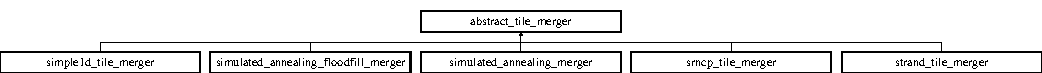
\includegraphics[height=0.978166cm]{classabstract__tile__merger}
\end{center}
\end{figure}
\subsection*{Public Member Functions}
\begin{DoxyCompactItemize}
\item 
\hyperlink{classabstract__tile__merger_a69c603d54ddfaf3346713756bfceaab5}{abstract\-\_\-tile\-\_\-merger} ()
\item 
virtual void \hyperlink{classabstract__tile__merger_a52ab494f77e495ab1a59b49e49c98db4}{merge\-\_\-tiles} (boost\-::shared\-\_\-ptr$<$ \hyperlink{classtiled__image}{tiled\-\_\-image} $>$ t)=0
\item 
virtual std\-::string \hyperlink{classabstract__tile__merger_a12ec9d118912b3c571d61ff9649042c6}{get\-\_\-name} ()=0
\item 
virtual void \hyperlink{classabstract__tile__merger_a7922b65624d12ef2d6c115218d2378b4}{usage\-\_\-help} ()=0
\end{DoxyCompactItemize}


\subsection{Detailed Description}
This pure virtual class provides an abstract interface for an merger that merges all tiles of a smart tiled image. It operates with boost smart pointers. 

\subsection{Constructor \& Destructor Documentation}
\hypertarget{classabstract__tile__merger_a69c603d54ddfaf3346713756bfceaab5}{\index{abstract\-\_\-tile\-\_\-merger@{abstract\-\_\-tile\-\_\-merger}!abstract\-\_\-tile\-\_\-merger@{abstract\-\_\-tile\-\_\-merger}}
\index{abstract\-\_\-tile\-\_\-merger@{abstract\-\_\-tile\-\_\-merger}!abstract_tile_merger@{abstract\-\_\-tile\-\_\-merger}}
\subsubsection[{abstract\-\_\-tile\-\_\-merger}]{\setlength{\rightskip}{0pt plus 5cm}abstract\-\_\-tile\-\_\-merger\-::abstract\-\_\-tile\-\_\-merger (
\begin{DoxyParamCaption}
{}
\end{DoxyParamCaption}
)\hspace{0.3cm}{\ttfamily [inline]}}}\label{classabstract__tile__merger_a69c603d54ddfaf3346713756bfceaab5}
Konstruktor 

\subsection{Member Function Documentation}
\hypertarget{classabstract__tile__merger_a12ec9d118912b3c571d61ff9649042c6}{\index{abstract\-\_\-tile\-\_\-merger@{abstract\-\_\-tile\-\_\-merger}!get\-\_\-name@{get\-\_\-name}}
\index{get\-\_\-name@{get\-\_\-name}!abstract_tile_merger@{abstract\-\_\-tile\-\_\-merger}}
\subsubsection[{get\-\_\-name}]{\setlength{\rightskip}{0pt plus 5cm}virtual std\-::string abstract\-\_\-tile\-\_\-merger\-::get\-\_\-name (
\begin{DoxyParamCaption}
{}
\end{DoxyParamCaption}
)\hspace{0.3cm}{\ttfamily [pure virtual]}}}\label{classabstract__tile__merger_a12ec9d118912b3c571d61ff9649042c6}
Return a name (with options) to set in the output file name 

Implemented in \hyperlink{classsimulated__annealing__floodfill__merger_a1e235b700efd2ccdcf771cd93251a1b9}{simulated\-\_\-annealing\-\_\-floodfill\-\_\-merger}, \hyperlink{classsimulated__annealing__merger_a2548233017acafb226be7bcdb2c91e22}{simulated\-\_\-annealing\-\_\-merger}, \hyperlink{classsrncp__tile__merger_a7e6fb5b07129a1354a8d997161b210c4}{srncp\-\_\-tile\-\_\-merger}, \hyperlink{classsimple1d__tile__merger_ac0810b20cdeb08613cb2a214267cf26a}{simple1d\-\_\-tile\-\_\-merger}, and \hyperlink{classstrand__tile__merger_a3e548d789df5b5a39435c095dd51365b}{strand\-\_\-tile\-\_\-merger}.

\hypertarget{classabstract__tile__merger_a52ab494f77e495ab1a59b49e49c98db4}{\index{abstract\-\_\-tile\-\_\-merger@{abstract\-\_\-tile\-\_\-merger}!merge\-\_\-tiles@{merge\-\_\-tiles}}
\index{merge\-\_\-tiles@{merge\-\_\-tiles}!abstract_tile_merger@{abstract\-\_\-tile\-\_\-merger}}
\subsubsection[{merge\-\_\-tiles}]{\setlength{\rightskip}{0pt plus 5cm}virtual void abstract\-\_\-tile\-\_\-merger\-::merge\-\_\-tiles (
\begin{DoxyParamCaption}
\item[{boost\-::shared\-\_\-ptr$<$ {\bf tiled\-\_\-image} $>$}]{t}
\end{DoxyParamCaption}
)\hspace{0.3cm}{\ttfamily [pure virtual]}}}\label{classabstract__tile__merger_a52ab494f77e495ab1a59b49e49c98db4}
Merge all given tiles inside the smart tiled image 
\begin{DoxyParams}{Parameters}
{\em t} & boost shared\-\_\-ptr to smart tiled image \\
\hline
\end{DoxyParams}


Implemented in \hyperlink{classsrncp__tile__merger_ad8330c73633437c5f4860d837bf63345}{srncp\-\_\-tile\-\_\-merger}, and \hyperlink{classsimple1d__tile__merger_ad73f710dd3ea0116859dcf2e5f6c5a14}{simple1d\-\_\-tile\-\_\-merger}.

\hypertarget{classabstract__tile__merger_a7922b65624d12ef2d6c115218d2378b4}{\index{abstract\-\_\-tile\-\_\-merger@{abstract\-\_\-tile\-\_\-merger}!usage\-\_\-help@{usage\-\_\-help}}
\index{usage\-\_\-help@{usage\-\_\-help}!abstract_tile_merger@{abstract\-\_\-tile\-\_\-merger}}
\subsubsection[{usage\-\_\-help}]{\setlength{\rightskip}{0pt plus 5cm}virtual void abstract\-\_\-tile\-\_\-merger\-::usage\-\_\-help (
\begin{DoxyParamCaption}
{}
\end{DoxyParamCaption}
)\hspace{0.3cm}{\ttfamily [pure virtual]}}}\label{classabstract__tile__merger_a7922b65624d12ef2d6c115218d2378b4}
Display a help on how to use this merger, in particular usage of merger-\/settings 

Implemented in \hyperlink{classsimulated__annealing__floodfill__merger_a6470774a227b289d5e16beac41e163d2}{simulated\-\_\-annealing\-\_\-floodfill\-\_\-merger}, \hyperlink{classsimulated__annealing__merger_a34ac2a006a40fe0b4e57c6868803bf07}{simulated\-\_\-annealing\-\_\-merger}, \hyperlink{classsrncp__tile__merger_ae57137ab8a1df19b86c28d3ff4aa1d9e}{srncp\-\_\-tile\-\_\-merger}, \hyperlink{classsimple1d__tile__merger_a4f18628ddf20f24efc13e705b469268c}{simple1d\-\_\-tile\-\_\-merger}, and \hyperlink{classstrand__tile__merger_af623214f3fe92b402d1a5510f1208071}{strand\-\_\-tile\-\_\-merger}.



The documentation for this class was generated from the following file\-:\begin{DoxyCompactItemize}
\item 
include/algorithm/abstract\-\_\-tile\-\_\-merger.\-h\end{DoxyCompactItemize}

\hypertarget{classabstract__tile__unwrapper}{\section{abstract\-\_\-tile\-\_\-unwrapper Class Reference}
\label{classabstract__tile__unwrapper}\index{abstract\-\_\-tile\-\_\-unwrapper@{abstract\-\_\-tile\-\_\-unwrapper}}
}


{\ttfamily \#include $<$abstract\-\_\-tile\-\_\-unwrapper.\-h$>$}

Inheritance diagram for abstract\-\_\-tile\-\_\-unwrapper\-:\begin{figure}[H]
\begin{center}
\leavevmode
\includegraphics[height=1.885522cm]{classabstract__tile__unwrapper}
\end{center}
\end{figure}
\subsection*{Public Member Functions}
\begin{DoxyCompactItemize}
\item 
\hyperlink{classabstract__tile__unwrapper_a31fc3a41d4adaab0ba7c2998e74ccedb}{abstract\-\_\-tile\-\_\-unwrapper} ()
\item 
virtual void \hyperlink{classabstract__tile__unwrapper_a74eedd36e55b9000b5986ff5980a563a}{unwrap} (boost\-::shared\-\_\-ptr$<$ \hyperlink{classtile}{tile} $>$ t)=0
\item 
virtual std\-::string \hyperlink{classabstract__tile__unwrapper_ae70f69a703e622e5ab13eabcc91fca4d}{get\-\_\-name} ()=0
\item 
virtual void \hyperlink{classabstract__tile__unwrapper_a469b36a7f302d5a2655631bbdb6f8daf}{usage\-\_\-help} ()=0
\end{DoxyCompactItemize}


\subsection{Detailed Description}
This pure virtual class provides an abstract interface for an unwrapper that unwraps a single tile. It operates with boost smart pointers. 

\subsection{Constructor \& Destructor Documentation}
\hypertarget{classabstract__tile__unwrapper_a31fc3a41d4adaab0ba7c2998e74ccedb}{\index{abstract\-\_\-tile\-\_\-unwrapper@{abstract\-\_\-tile\-\_\-unwrapper}!abstract\-\_\-tile\-\_\-unwrapper@{abstract\-\_\-tile\-\_\-unwrapper}}
\index{abstract\-\_\-tile\-\_\-unwrapper@{abstract\-\_\-tile\-\_\-unwrapper}!abstract_tile_unwrapper@{abstract\-\_\-tile\-\_\-unwrapper}}
\subsubsection[{abstract\-\_\-tile\-\_\-unwrapper}]{\setlength{\rightskip}{0pt plus 5cm}abstract\-\_\-tile\-\_\-unwrapper\-::abstract\-\_\-tile\-\_\-unwrapper (
\begin{DoxyParamCaption}
{}
\end{DoxyParamCaption}
)\hspace{0.3cm}{\ttfamily [inline]}}}\label{classabstract__tile__unwrapper_a31fc3a41d4adaab0ba7c2998e74ccedb}
Konstruktor 

\subsection{Member Function Documentation}
\hypertarget{classabstract__tile__unwrapper_ae70f69a703e622e5ab13eabcc91fca4d}{\index{abstract\-\_\-tile\-\_\-unwrapper@{abstract\-\_\-tile\-\_\-unwrapper}!get\-\_\-name@{get\-\_\-name}}
\index{get\-\_\-name@{get\-\_\-name}!abstract_tile_unwrapper@{abstract\-\_\-tile\-\_\-unwrapper}}
\subsubsection[{get\-\_\-name}]{\setlength{\rightskip}{0pt plus 5cm}virtual std\-::string abstract\-\_\-tile\-\_\-unwrapper\-::get\-\_\-name (
\begin{DoxyParamCaption}
{}
\end{DoxyParamCaption}
)\hspace{0.3cm}{\ttfamily [pure virtual]}}}\label{classabstract__tile__unwrapper_ae70f69a703e622e5ab13eabcc91fca4d}
Return a name (with options) to set in the output file name 

Implemented in \hyperlink{classleast__squares__grad__unwrapper_af66d1a659d6cfbb82200d120f43dd939}{least\-\_\-squares\-\_\-grad\-\_\-unwrapper}, \hyperlink{classstrand__tile__unwrapper_ae4ce9d7459840ada66b7492ea2873969}{strand\-\_\-tile\-\_\-unwrapper}, and \hyperlink{classgrad__fit__tile__unwrapper_a46a71a2adc53411289f792aae8c1b61c}{grad\-\_\-fit\-\_\-tile\-\_\-unwrapper}.

\hypertarget{classabstract__tile__unwrapper_a74eedd36e55b9000b5986ff5980a563a}{\index{abstract\-\_\-tile\-\_\-unwrapper@{abstract\-\_\-tile\-\_\-unwrapper}!unwrap@{unwrap}}
\index{unwrap@{unwrap}!abstract_tile_unwrapper@{abstract\-\_\-tile\-\_\-unwrapper}}
\subsubsection[{unwrap}]{\setlength{\rightskip}{0pt plus 5cm}virtual void abstract\-\_\-tile\-\_\-unwrapper\-::unwrap (
\begin{DoxyParamCaption}
\item[{boost\-::shared\-\_\-ptr$<$ {\bf tile} $>$}]{t}
\end{DoxyParamCaption}
)\hspace{0.3cm}{\ttfamily [pure virtual]}}}\label{classabstract__tile__unwrapper_a74eedd36e55b9000b5986ff5980a563a}
Unwrap a given tile. 
\begin{DoxyParams}{Parameters}
{\em t} & \\
\hline
\end{DoxyParams}


Implemented in \hyperlink{classstrand__tile__unwrapper_a520d7832e80746c9996fe042b5993235}{strand\-\_\-tile\-\_\-unwrapper}.

\hypertarget{classabstract__tile__unwrapper_a469b36a7f302d5a2655631bbdb6f8daf}{\index{abstract\-\_\-tile\-\_\-unwrapper@{abstract\-\_\-tile\-\_\-unwrapper}!usage\-\_\-help@{usage\-\_\-help}}
\index{usage\-\_\-help@{usage\-\_\-help}!abstract_tile_unwrapper@{abstract\-\_\-tile\-\_\-unwrapper}}
\subsubsection[{usage\-\_\-help}]{\setlength{\rightskip}{0pt plus 5cm}virtual void abstract\-\_\-tile\-\_\-unwrapper\-::usage\-\_\-help (
\begin{DoxyParamCaption}
{}
\end{DoxyParamCaption}
)\hspace{0.3cm}{\ttfamily [pure virtual]}}}\label{classabstract__tile__unwrapper_a469b36a7f302d5a2655631bbdb6f8daf}
Display a help on how to use this merger, in particular usage of merger-\/settings 

Implemented in \hyperlink{classleast__squares__grad__unwrapper_a8795b4b968a336d28a81e910cbc9f4ab}{least\-\_\-squares\-\_\-grad\-\_\-unwrapper}, \hyperlink{classstrand__tile__unwrapper_aebfdb44f1be923a6528471ea38174669}{strand\-\_\-tile\-\_\-unwrapper}, and \hyperlink{classgrad__fit__tile__unwrapper_a62df2a6e799306b85f273a4f5aa43b4c}{grad\-\_\-fit\-\_\-tile\-\_\-unwrapper}.



The documentation for this class was generated from the following file\-:\begin{DoxyCompactItemize}
\item 
include/algorithm/abstract\-\_\-tile\-\_\-unwrapper.\-h\end{DoxyCompactItemize}

\hypertarget{classabstract__unwrapper}{\section{abstract\-\_\-unwrapper Class Reference}
\label{classabstract__unwrapper}\index{abstract\-\_\-unwrapper@{abstract\-\_\-unwrapper}}
}


{\ttfamily \#include $<$abstract\-\_\-unwrapper.\-h$>$}

Inheritance diagram for abstract\-\_\-unwrapper\-:\begin{figure}[H]
\begin{center}
\leavevmode
\includegraphics[height=2.000000cm]{classabstract__unwrapper}
\end{center}
\end{figure}
\subsection*{Public Member Functions}
\begin{DoxyCompactItemize}
\item 
virtual boost\-::shared\-\_\-ptr\\*
$<$ \hyperlink{classfloat__image}{float\-\_\-image} $>$ \hyperlink{classabstract__unwrapper_af7d5640f6f7e8beb7f7829c2260b94ee}{unwrap} (boost\-::shared\-\_\-ptr$<$ \hyperlink{classfloat__image}{float\-\_\-image} $>$ wrapped\-\_\-phase\-\_\-image)=0
\end{DoxyCompactItemize}


\subsection{Detailed Description}
This pure virtual class provides an interface for a general unwrapper that operates with boost smart pointers. 

\subsection{Member Function Documentation}
\hypertarget{classabstract__unwrapper_af7d5640f6f7e8beb7f7829c2260b94ee}{\index{abstract\-\_\-unwrapper@{abstract\-\_\-unwrapper}!unwrap@{unwrap}}
\index{unwrap@{unwrap}!abstract_unwrapper@{abstract\-\_\-unwrapper}}
\subsubsection[{unwrap}]{\setlength{\rightskip}{0pt plus 5cm}virtual boost\-::shared\-\_\-ptr$<${\bf float\-\_\-image}$>$ abstract\-\_\-unwrapper\-::unwrap (
\begin{DoxyParamCaption}
\item[{boost\-::shared\-\_\-ptr$<$ {\bf float\-\_\-image} $>$}]{wrapped\-\_\-phase\-\_\-image}
\end{DoxyParamCaption}
)\hspace{0.3cm}{\ttfamily [pure virtual]}}}\label{classabstract__unwrapper_af7d5640f6f7e8beb7f7829c2260b94ee}
An asbtract method for phase unwrapping. 
\begin{DoxyParams}{Parameters}
{\em wrapped\-\_\-phase\-\_\-image} & This image contains the wrapped phase data. \\
\hline
\end{DoxyParams}
\begin{DoxyReturn}{Returns}
A \hyperlink{classfloat__image}{float\-\_\-image} with the unwrapped phase data. The image will actually be a \hyperlink{classrow__major__float__image}{row\-\_\-major\-\_\-float\-\_\-image}. 
\end{DoxyReturn}


Implemented in \hyperlink{classpx__floodfill__sim__ann__unwrapper_a72c5c9cb7f151f50042b3d17f8b10b79}{px\-\_\-floodfill\-\_\-sim\-\_\-ann\-\_\-unwrapper}.



The documentation for this class was generated from the following file\-:\begin{DoxyCompactItemize}
\item 
include/algorithm/abstract\-\_\-unwrapper.\-h\end{DoxyCompactItemize}

\hypertarget{classcol__major__float__image}{\section{col\-\_\-major\-\_\-float\-\_\-image Class Reference}
\label{classcol__major__float__image}\index{col\-\_\-major\-\_\-float\-\_\-image@{col\-\_\-major\-\_\-float\-\_\-image}}
}
Inheritance diagram for col\-\_\-major\-\_\-float\-\_\-image\-:\begin{figure}[H]
\begin{center}
\leavevmode
\includegraphics[height=2.000000cm]{classcol__major__float__image}
\end{center}
\end{figure}
\subsection*{Public Member Functions}
\begin{DoxyCompactItemize}
\item 
\hypertarget{classcol__major__float__image_afcf4d9a3059aca06c840338665077b53}{{\bfseries col\-\_\-major\-\_\-float\-\_\-image} (float $\ast$data, long width, long height)}\label{classcol__major__float__image_afcf4d9a3059aca06c840338665077b53}

\item 
\hyperlink{classcol__major__float__image_adeaacc7a78c0e3448597b34bff5b4c62}{col\-\_\-major\-\_\-float\-\_\-image} (long width, long height)
\item 
virtual float \& \hyperlink{classcol__major__float__image_a45315790d78a3d27559946f198129708}{operator()} (long w, long h)
\item 
\hypertarget{classcol__major__float__image_a83784cb35e0fef47a5f4b68fcf5a35c6}{virtual float {\bfseries operator()} (long w, long h) const }\label{classcol__major__float__image_a83784cb35e0fef47a5f4b68fcf5a35c6}

\end{DoxyCompactItemize}
\subsection*{Additional Inherited Members}


\subsection{Constructor \& Destructor Documentation}
\hypertarget{classcol__major__float__image_adeaacc7a78c0e3448597b34bff5b4c62}{\index{col\-\_\-major\-\_\-float\-\_\-image@{col\-\_\-major\-\_\-float\-\_\-image}!col\-\_\-major\-\_\-float\-\_\-image@{col\-\_\-major\-\_\-float\-\_\-image}}
\index{col\-\_\-major\-\_\-float\-\_\-image@{col\-\_\-major\-\_\-float\-\_\-image}!col_major_float_image@{col\-\_\-major\-\_\-float\-\_\-image}}
\subsubsection[{col\-\_\-major\-\_\-float\-\_\-image}]{\setlength{\rightskip}{0pt plus 5cm}col\-\_\-major\-\_\-float\-\_\-image\-::col\-\_\-major\-\_\-float\-\_\-image (
\begin{DoxyParamCaption}
\item[{long}]{width, }
\item[{long}]{height}
\end{DoxyParamCaption}
)\hspace{0.3cm}{\ttfamily [inline]}}}\label{classcol__major__float__image_adeaacc7a78c0e3448597b34bff5b4c62}
Generate image that reserves memory 
\begin{DoxyParams}{Parameters}
{\em width} & \\
\hline
{\em height} & \\
\hline
\end{DoxyParams}


\subsection{Member Function Documentation}
\hypertarget{classcol__major__float__image_a45315790d78a3d27559946f198129708}{\index{col\-\_\-major\-\_\-float\-\_\-image@{col\-\_\-major\-\_\-float\-\_\-image}!operator()@{operator()}}
\index{operator()@{operator()}!col_major_float_image@{col\-\_\-major\-\_\-float\-\_\-image}}
\subsubsection[{operator()}]{\setlength{\rightskip}{0pt plus 5cm}virtual float\& col\-\_\-major\-\_\-float\-\_\-image\-::operator() (
\begin{DoxyParamCaption}
\item[{long}]{w, }
\item[{long}]{h}
\end{DoxyParamCaption}
)\hspace{0.3cm}{\ttfamily [inline]}, {\ttfamily [virtual]}}}\label{classcol__major__float__image_a45315790d78a3d27559946f198129708}
Return element at position width = w, height = h, starting with (0,0) in upper left corner of the image. Implemented in child classes, see e.\-g. \hyperlink{classrow__major__float__image}{row\-\_\-major\-\_\-float\-\_\-image}. 

Implements \hyperlink{classfloat__image_a62e1446efb51fadcfeebf50568f9d1e9}{float\-\_\-image}.



The documentation for this class was generated from the following file\-:\begin{DoxyCompactItemize}
\item 
include/image/col\-\_\-major\-\_\-image.\-h\end{DoxyCompactItemize}

\input{class_ui_1_1digiholo_main_gui}
\input{classdigiholo_main_gui}
\hypertarget{struct_e_d_g_e}{\section{E\-D\-G\-E Struct Reference}
\label{struct_e_d_g_e}\index{E\-D\-G\-E@{E\-D\-G\-E}}
}
\subsection*{Public Attributes}
\begin{DoxyCompactItemize}
\item 
\hypertarget{struct_e_d_g_e_aeb147494099907a93ab92933235b5b2e}{float {\bfseries reliab}}\label{struct_e_d_g_e_aeb147494099907a93ab92933235b5b2e}

\item 
\hypertarget{struct_e_d_g_e_ab82d5a09f9a58543da71f2e8cbc821aa}{\hyperlink{struct_p_i_x_e_l}{P\-I\-X\-E\-L} $\ast$ {\bfseries pointer\-\_\-1}}\label{struct_e_d_g_e_ab82d5a09f9a58543da71f2e8cbc821aa}

\item 
\hypertarget{struct_e_d_g_e_a06ed3287e2c03f8b13d94b0845e065db}{\hyperlink{struct_p_i_x_e_l}{P\-I\-X\-E\-L} $\ast$ {\bfseries pointer\-\_\-2}}\label{struct_e_d_g_e_a06ed3287e2c03f8b13d94b0845e065db}

\item 
\hypertarget{struct_e_d_g_e_a29dca15549696bdc742e37df73de3482}{int {\bfseries increment}}\label{struct_e_d_g_e_a29dca15549696bdc742e37df73de3482}

\end{DoxyCompactItemize}


The documentation for this struct was generated from the following file\-:\begin{DoxyCompactItemize}
\item 
include/srncp/srncp\-\_\-unwrap.\-h\end{DoxyCompactItemize}

\hypertarget{classfloat__image}{\section{float\-\_\-image Class Reference}
\label{classfloat__image}\index{float\-\_\-image@{float\-\_\-image}}
}
Inheritance diagram for float\-\_\-image\-:\begin{figure}[H]
\begin{center}
\leavevmode
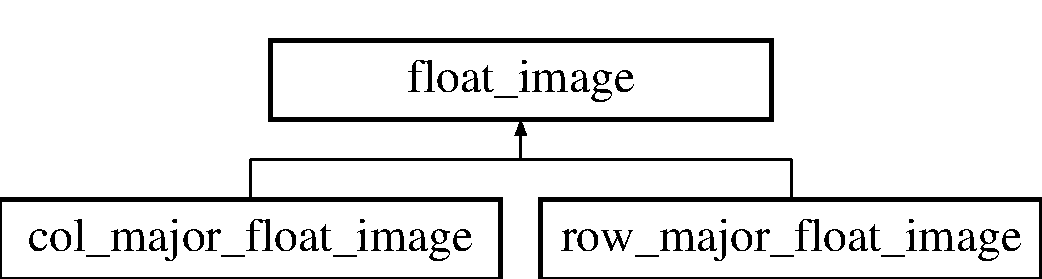
\includegraphics[height=2.000000cm]{classfloat__image}
\end{center}
\end{figure}
\subsection*{Public Member Functions}
\begin{DoxyCompactItemize}
\item 
\hyperlink{classfloat__image_a9e4ea7f98eb8c33e025cd21d61703c66}{float\-\_\-image} (long width, long height)
\item 
\hyperlink{classfloat__image_a4626247e8da835a5be04e346b577f85e}{float\-\_\-image} (float $\ast$data, long width, long height)
\item 
virtual long \hyperlink{classfloat__image_a08ba5e995f656dfebc5aaad0a9be390c}{get\-\_\-width} () const 
\item 
virtual long \hyperlink{classfloat__image_aeab41642909a0ee8d6e0ffcc2e7287b1}{get\-\_\-height} () const 
\item 
virtual float $\ast$ \hyperlink{classfloat__image_ab6dbf1f20614ba84f7b8f2c01b7aa3da}{get\-\_\-data\-\_\-pointer} ()
\item 
virtual float \& \hyperlink{classfloat__image_a62e1446efb51fadcfeebf50568f9d1e9}{operator()} (long w, long h)=0
\item 
\hypertarget{classfloat__image_ae3ae19180d1903bdeb0ffdb6f509a9f5}{virtual float {\bfseries operator()} (long w, long h) const =0}\label{classfloat__image_ae3ae19180d1903bdeb0ffdb6f509a9f5}

\item 
virtual void \hyperlink{classfloat__image_adffd8782a04ea4d764865aace1e43c93}{zero\-\_\-fill} ()
\item 
virtual bool \hyperlink{classfloat__image_a9cead12d50823ca313f6b7b16a57b092}{copy\-\_\-data\-\_\-to} (\hyperlink{classfloat__image}{float\-\_\-image} $\ast$img)
\item 
virtual void \hyperlink{classfloat__image_a3ef2df1d69f6791d2bef54636b625f82}{clear\-\_\-mem} ()
\item 
virtual float \hyperlink{classfloat__image_a53701b38abc94f8a707e8ceb2e6e71da}{get\-\_\-pixel} (long iw, long ih)
\item 
virtual void \hyperlink{classfloat__image_a97b520fc634fc4eb1930491b74d1f79b}{set\-\_\-pixel} (long iw, long ih, float val)
\end{DoxyCompactItemize}
\subsection*{Protected Attributes}
\begin{DoxyCompactItemize}
\item 
\hypertarget{classfloat__image_a43df6eebb483b16921cee23e80f61f5b}{float $\ast$ {\bfseries data}}\label{classfloat__image_a43df6eebb483b16921cee23e80f61f5b}

\item 
\hypertarget{classfloat__image_a92e539199f8cfa3c8ece64e2bdca54c7}{long {\bfseries width}}\label{classfloat__image_a92e539199f8cfa3c8ece64e2bdca54c7}

\item 
\hypertarget{classfloat__image_af7c859a1a77e6886adff0fd47976d069}{long {\bfseries height}}\label{classfloat__image_af7c859a1a77e6886adff0fd47976d069}

\end{DoxyCompactItemize}


\subsection{Detailed Description}
speichert ein 2\-D Bild, welches in einem 1\-D Datenvektor gespeichert wird. Die Ordnung des Datenvektors gibt die Klasse nicht vor. Es müssen auch nicht alle Daten hintereinander weg liegen. Die Zugriffsoperatoren sollen überladen werden, um eine bestimmte Art der Speicherung (z.\-b. row-\/major / column-\/major) oder sonstwas zu abstrahieren. Wichtig\-: Beim Aufruf des Destruktors des Bildes wird das entsprechende Array nicht freigegeben! 

\subsection{Constructor \& Destructor Documentation}
\hypertarget{classfloat__image_a9e4ea7f98eb8c33e025cd21d61703c66}{\index{float\-\_\-image@{float\-\_\-image}!float\-\_\-image@{float\-\_\-image}}
\index{float\-\_\-image@{float\-\_\-image}!float_image@{float\-\_\-image}}
\subsubsection[{float\-\_\-image}]{\setlength{\rightskip}{0pt plus 5cm}float\-\_\-image\-::float\-\_\-image (
\begin{DoxyParamCaption}
\item[{long}]{width, }
\item[{long}]{height}
\end{DoxyParamCaption}
)}}\label{classfloat__image_a9e4ea7f98eb8c33e025cd21d61703c66}
Create float image with and allocate data array! The data will not be zero filled. 
\begin{DoxyParams}{Parameters}
{\em width} & \\
\hline
{\em height} & \\
\hline
\end{DoxyParams}
\hypertarget{classfloat__image_a4626247e8da835a5be04e346b577f85e}{\index{float\-\_\-image@{float\-\_\-image}!float\-\_\-image@{float\-\_\-image}}
\index{float\-\_\-image@{float\-\_\-image}!float_image@{float\-\_\-image}}
\subsubsection[{float\-\_\-image}]{\setlength{\rightskip}{0pt plus 5cm}float\-\_\-image\-::float\-\_\-image (
\begin{DoxyParamCaption}
\item[{float $\ast$}]{data, }
\item[{long}]{width, }
\item[{long}]{height}
\end{DoxyParamCaption}
)}}\label{classfloat__image_a4626247e8da835a5be04e346b577f85e}
Create float image with specified data array. The image will operate on this array. 
\begin{DoxyParams}{Parameters}
{\em data} & \\
\hline
{\em width} & \\
\hline
{\em height} & \\
\hline
\end{DoxyParams}


\subsection{Member Function Documentation}
\hypertarget{classfloat__image_a3ef2df1d69f6791d2bef54636b625f82}{\index{float\-\_\-image@{float\-\_\-image}!clear\-\_\-mem@{clear\-\_\-mem}}
\index{clear\-\_\-mem@{clear\-\_\-mem}!float_image@{float\-\_\-image}}
\subsubsection[{clear\-\_\-mem}]{\setlength{\rightskip}{0pt plus 5cm}void float\-\_\-image\-::clear\-\_\-mem (
\begin{DoxyParamCaption}
{}
\end{DoxyParamCaption}
)\hspace{0.3cm}{\ttfamily [virtual]}}}\label{classfloat__image_a3ef2df1d69f6791d2bef54636b625f82}
Free memory associated with the image. This is not done when the destructor is called. \hypertarget{classfloat__image_a9cead12d50823ca313f6b7b16a57b092}{\index{float\-\_\-image@{float\-\_\-image}!copy\-\_\-data\-\_\-to@{copy\-\_\-data\-\_\-to}}
\index{copy\-\_\-data\-\_\-to@{copy\-\_\-data\-\_\-to}!float_image@{float\-\_\-image}}
\subsubsection[{copy\-\_\-data\-\_\-to}]{\setlength{\rightskip}{0pt plus 5cm}bool float\-\_\-image\-::copy\-\_\-data\-\_\-to (
\begin{DoxyParamCaption}
\item[{{\bf float\-\_\-image} $\ast$}]{img}
\end{DoxyParamCaption}
)\hspace{0.3cm}{\ttfamily [virtual]}}}\label{classfloat__image_a9cead12d50823ca313f6b7b16a57b092}
Copies the data from this image into the given image. Both images need to have the same dimensions. 
\begin{DoxyParams}{Parameters}
{\em img} & Data from this image is copied into img. \\
\hline
\end{DoxyParams}
\begin{DoxyReturn}{Returns}
true if successful, false if not. 
\end{DoxyReturn}
\hypertarget{classfloat__image_ab6dbf1f20614ba84f7b8f2c01b7aa3da}{\index{float\-\_\-image@{float\-\_\-image}!get\-\_\-data\-\_\-pointer@{get\-\_\-data\-\_\-pointer}}
\index{get\-\_\-data\-\_\-pointer@{get\-\_\-data\-\_\-pointer}!float_image@{float\-\_\-image}}
\subsubsection[{get\-\_\-data\-\_\-pointer}]{\setlength{\rightskip}{0pt plus 5cm}float $\ast$ float\-\_\-image\-::get\-\_\-data\-\_\-pointer (
\begin{DoxyParamCaption}
{}
\end{DoxyParamCaption}
)\hspace{0.3cm}{\ttfamily [virtual]}}}\label{classfloat__image_ab6dbf1f20614ba84f7b8f2c01b7aa3da}
\begin{DoxyReturn}{Returns}
pointer to data array 
\end{DoxyReturn}
\hypertarget{classfloat__image_aeab41642909a0ee8d6e0ffcc2e7287b1}{\index{float\-\_\-image@{float\-\_\-image}!get\-\_\-height@{get\-\_\-height}}
\index{get\-\_\-height@{get\-\_\-height}!float_image@{float\-\_\-image}}
\subsubsection[{get\-\_\-height}]{\setlength{\rightskip}{0pt plus 5cm}long float\-\_\-image\-::get\-\_\-height (
\begin{DoxyParamCaption}
{}
\end{DoxyParamCaption}
) const\hspace{0.3cm}{\ttfamily [virtual]}}}\label{classfloat__image_aeab41642909a0ee8d6e0ffcc2e7287b1}
\begin{DoxyReturn}{Returns}
image height 
\end{DoxyReturn}
\hypertarget{classfloat__image_a53701b38abc94f8a707e8ceb2e6e71da}{\index{float\-\_\-image@{float\-\_\-image}!get\-\_\-pixel@{get\-\_\-pixel}}
\index{get\-\_\-pixel@{get\-\_\-pixel}!float_image@{float\-\_\-image}}
\subsubsection[{get\-\_\-pixel}]{\setlength{\rightskip}{0pt plus 5cm}float float\-\_\-image\-::get\-\_\-pixel (
\begin{DoxyParamCaption}
\item[{long}]{iw, }
\item[{long}]{ih}
\end{DoxyParamCaption}
)\hspace{0.3cm}{\ttfamily [virtual]}}}\label{classfloat__image_a53701b38abc94f8a707e8ceb2e6e71da}
Get Pixel value at specified position. 
\begin{DoxyParams}{Parameters}
{\em iw} & \\
\hline
{\em ih} & \\
\hline
\end{DoxyParams}
\begin{DoxyReturn}{Returns}

\end{DoxyReturn}
\hypertarget{classfloat__image_a08ba5e995f656dfebc5aaad0a9be390c}{\index{float\-\_\-image@{float\-\_\-image}!get\-\_\-width@{get\-\_\-width}}
\index{get\-\_\-width@{get\-\_\-width}!float_image@{float\-\_\-image}}
\subsubsection[{get\-\_\-width}]{\setlength{\rightskip}{0pt plus 5cm}long float\-\_\-image\-::get\-\_\-width (
\begin{DoxyParamCaption}
{}
\end{DoxyParamCaption}
) const\hspace{0.3cm}{\ttfamily [virtual]}}}\label{classfloat__image_a08ba5e995f656dfebc5aaad0a9be390c}
\begin{DoxyReturn}{Returns}
image width 
\end{DoxyReturn}
\hypertarget{classfloat__image_a62e1446efb51fadcfeebf50568f9d1e9}{\index{float\-\_\-image@{float\-\_\-image}!operator()@{operator()}}
\index{operator()@{operator()}!float_image@{float\-\_\-image}}
\subsubsection[{operator()}]{\setlength{\rightskip}{0pt plus 5cm}virtual float\& float\-\_\-image\-::operator() (
\begin{DoxyParamCaption}
\item[{long}]{w, }
\item[{long}]{h}
\end{DoxyParamCaption}
)\hspace{0.3cm}{\ttfamily [pure virtual]}}}\label{classfloat__image_a62e1446efb51fadcfeebf50568f9d1e9}
Return element at position width = w, height = h, starting with (0,0) in upper left corner of the image. Implemented in child classes, see e.\-g. \hyperlink{classrow__major__float__image}{row\-\_\-major\-\_\-float\-\_\-image}. 

Implemented in \hyperlink{classcol__major__float__image_a45315790d78a3d27559946f198129708}{col\-\_\-major\-\_\-float\-\_\-image}, and \hyperlink{classrow__major__float__image_a04b9b253a3771e0963c839a9a85ccd99}{row\-\_\-major\-\_\-float\-\_\-image}.

\hypertarget{classfloat__image_a97b520fc634fc4eb1930491b74d1f79b}{\index{float\-\_\-image@{float\-\_\-image}!set\-\_\-pixel@{set\-\_\-pixel}}
\index{set\-\_\-pixel@{set\-\_\-pixel}!float_image@{float\-\_\-image}}
\subsubsection[{set\-\_\-pixel}]{\setlength{\rightskip}{0pt plus 5cm}void float\-\_\-image\-::set\-\_\-pixel (
\begin{DoxyParamCaption}
\item[{long}]{iw, }
\item[{long}]{ih, }
\item[{float}]{val}
\end{DoxyParamCaption}
)\hspace{0.3cm}{\ttfamily [virtual]}}}\label{classfloat__image_a97b520fc634fc4eb1930491b74d1f79b}
Set Pixel value at specified position. 
\begin{DoxyParams}{Parameters}
{\em iw} & \\
\hline
{\em ih} & \\
\hline
{\em val} & \\
\hline
\end{DoxyParams}
\begin{DoxyReturn}{Returns}

\end{DoxyReturn}
\hypertarget{classfloat__image_adffd8782a04ea4d764865aace1e43c93}{\index{float\-\_\-image@{float\-\_\-image}!zero\-\_\-fill@{zero\-\_\-fill}}
\index{zero\-\_\-fill@{zero\-\_\-fill}!float_image@{float\-\_\-image}}
\subsubsection[{zero\-\_\-fill}]{\setlength{\rightskip}{0pt plus 5cm}void float\-\_\-image\-::zero\-\_\-fill (
\begin{DoxyParamCaption}
{}
\end{DoxyParamCaption}
)\hspace{0.3cm}{\ttfamily [virtual]}}}\label{classfloat__image_adffd8782a04ea4d764865aace1e43c93}
Fill image with zeroes. 

The documentation for this class was generated from the following files\-:\begin{DoxyCompactItemize}
\item 
include/float\-\_\-image.\-h\item 
src/float\-\_\-image.\-cpp\end{DoxyCompactItemize}

\hypertarget{classgrad__fit__tile__unwrapper}{\section{grad\-\_\-fit\-\_\-tile\-\_\-unwrapper Class Reference}
\label{classgrad__fit__tile__unwrapper}\index{grad\-\_\-fit\-\_\-tile\-\_\-unwrapper@{grad\-\_\-fit\-\_\-tile\-\_\-unwrapper}}
}
Inheritance diagram for grad\-\_\-fit\-\_\-tile\-\_\-unwrapper\-:\begin{figure}[H]
\begin{center}
\leavevmode
\includegraphics[height=2.000000cm]{classgrad__fit__tile__unwrapper}
\end{center}
\end{figure}
\subsection*{Public Member Functions}
\begin{DoxyCompactItemize}
\item 
\hypertarget{classgrad__fit__tile__unwrapper_a79033def7d478d1ef50b627b0663700d}{void {\bfseries unwrap} (sharedptr$<$ \hyperlink{classtile}{tile} $>$ t)}\label{classgrad__fit__tile__unwrapper_a79033def7d478d1ef50b627b0663700d}

\item 
virtual std\-::string \hyperlink{classgrad__fit__tile__unwrapper_a46a71a2adc53411289f792aae8c1b61c}{get\-\_\-name} ()
\item 
virtual void \hyperlink{classgrad__fit__tile__unwrapper_a62df2a6e799306b85f273a4f5aa43b4c}{usage\-\_\-help} ()
\end{DoxyCompactItemize}


\subsection{Member Function Documentation}
\hypertarget{classgrad__fit__tile__unwrapper_a46a71a2adc53411289f792aae8c1b61c}{\index{grad\-\_\-fit\-\_\-tile\-\_\-unwrapper@{grad\-\_\-fit\-\_\-tile\-\_\-unwrapper}!get\-\_\-name@{get\-\_\-name}}
\index{get\-\_\-name@{get\-\_\-name}!grad_fit_tile_unwrapper@{grad\-\_\-fit\-\_\-tile\-\_\-unwrapper}}
\subsubsection[{get\-\_\-name}]{\setlength{\rightskip}{0pt plus 5cm}std\-::string grad\-\_\-fit\-\_\-tile\-\_\-unwrapper\-::get\-\_\-name (
\begin{DoxyParamCaption}
{}
\end{DoxyParamCaption}
)\hspace{0.3cm}{\ttfamily [virtual]}}}\label{classgrad__fit__tile__unwrapper_a46a71a2adc53411289f792aae8c1b61c}
Return a name (with options) to set in the output file name 

Implements \hyperlink{classabstract__tile__unwrapper_ae70f69a703e622e5ab13eabcc91fca4d}{abstract\-\_\-tile\-\_\-unwrapper}.

\hypertarget{classgrad__fit__tile__unwrapper_a62df2a6e799306b85f273a4f5aa43b4c}{\index{grad\-\_\-fit\-\_\-tile\-\_\-unwrapper@{grad\-\_\-fit\-\_\-tile\-\_\-unwrapper}!usage\-\_\-help@{usage\-\_\-help}}
\index{usage\-\_\-help@{usage\-\_\-help}!grad_fit_tile_unwrapper@{grad\-\_\-fit\-\_\-tile\-\_\-unwrapper}}
\subsubsection[{usage\-\_\-help}]{\setlength{\rightskip}{0pt plus 5cm}void grad\-\_\-fit\-\_\-tile\-\_\-unwrapper\-::usage\-\_\-help (
\begin{DoxyParamCaption}
{}
\end{DoxyParamCaption}
)\hspace{0.3cm}{\ttfamily [virtual]}}}\label{classgrad__fit__tile__unwrapper_a62df2a6e799306b85f273a4f5aa43b4c}
Display a help on how to use this merger, in particular usage of merger-\/settings 

Implements \hyperlink{classabstract__tile__unwrapper_a469b36a7f302d5a2655631bbdb6f8daf}{abstract\-\_\-tile\-\_\-unwrapper}.



The documentation for this class was generated from the following files\-:\begin{DoxyCompactItemize}
\item 
include/algorithm/grad\-\_\-fit\-\_\-tile\-\_\-unwrapper.\-h\item 
src/algorithm/grad\-\_\-fit\-\_\-tile\-\_\-unwrapper.\-cpp\end{DoxyCompactItemize}

\hypertarget{classminimization__tile__unwrapper}{\section{minimization\-\_\-tile\-\_\-unwrapper Class Reference}
\label{classminimization__tile__unwrapper}\index{minimization\-\_\-tile\-\_\-unwrapper@{minimization\-\_\-tile\-\_\-unwrapper}}
}
Inheritance diagram for minimization\-\_\-tile\-\_\-unwrapper\-:\begin{figure}[H]
\begin{center}
\leavevmode
\includegraphics[height=2.000000cm]{classminimization__tile__unwrapper}
\end{center}
\end{figure}
\subsection*{Public Member Functions}
\begin{DoxyCompactItemize}
\item 
\hyperlink{classminimization__tile__unwrapper_acd1f71bbf4da842023eeb888ff07df07}{minimization\-\_\-tile\-\_\-unwrapper} (int max\-\_\-inter, float tol=0.\-0314)
\item 
virtual \hyperlink{classminimization__tile__unwrapper_a87733a219fdd57965ecccf833d6d8ea7}{$\sim$minimization\-\_\-tile\-\_\-unwrapper} ()
\item 
virtual void \hyperlink{classminimization__tile__unwrapper_a029e05336da3208ecb7a00ab553dd1c1}{unwrap} (\hyperlink{classtile}{tile} $\ast$t)
\end{DoxyCompactItemize}


\subsection{Detailed Description}
!! Diese Klasse soll mit G\-S\-L eine effizienteren Tile-\/\-Unwrap als der \hyperlink{class_strand__tile__unwrapper}{Strand\-\_\-tile\-\_\-unwrapper} durchführen. Es ist allerdings nicht so leicht, das Minimierungsproblem so zu verpacken, dass es mit Minimierungsroutinen gelöst werden kann. Man muss erstmal das Minimum eingrenzen... wie soll ich das möglichst effizient machen? 

\subsection{Constructor \& Destructor Documentation}
\hypertarget{classminimization__tile__unwrapper_acd1f71bbf4da842023eeb888ff07df07}{\index{minimization\-\_\-tile\-\_\-unwrapper@{minimization\-\_\-tile\-\_\-unwrapper}!minimization\-\_\-tile\-\_\-unwrapper@{minimization\-\_\-tile\-\_\-unwrapper}}
\index{minimization\-\_\-tile\-\_\-unwrapper@{minimization\-\_\-tile\-\_\-unwrapper}!minimization_tile_unwrapper@{minimization\-\_\-tile\-\_\-unwrapper}}
\subsubsection[{minimization\-\_\-tile\-\_\-unwrapper}]{\setlength{\rightskip}{0pt plus 5cm}minimization\-\_\-tile\-\_\-unwrapper\-::minimization\-\_\-tile\-\_\-unwrapper (
\begin{DoxyParamCaption}
\item[{int}]{max\-\_\-inter, }
\item[{float}]{tol = {\ttfamily 0.0314}}
\end{DoxyParamCaption}
)}}\label{classminimization__tile__unwrapper_acd1f71bbf4da842023eeb888ff07df07}
Constructor 
\begin{DoxyParams}{Parameters}
{\em max\-\_\-inter} & Max number of iterations for minimization \\
\hline
{\em tol} & Tolerance parameter as stopping criterion for minimization \\
\hline
\end{DoxyParams}
Allocate a Brent type minimizer; \hypertarget{classminimization__tile__unwrapper_a87733a219fdd57965ecccf833d6d8ea7}{\index{minimization\-\_\-tile\-\_\-unwrapper@{minimization\-\_\-tile\-\_\-unwrapper}!$\sim$minimization\-\_\-tile\-\_\-unwrapper@{$\sim$minimization\-\_\-tile\-\_\-unwrapper}}
\index{$\sim$minimization\-\_\-tile\-\_\-unwrapper@{$\sim$minimization\-\_\-tile\-\_\-unwrapper}!minimization_tile_unwrapper@{minimization\-\_\-tile\-\_\-unwrapper}}
\subsubsection[{$\sim$minimization\-\_\-tile\-\_\-unwrapper}]{\setlength{\rightskip}{0pt plus 5cm}minimization\-\_\-tile\-\_\-unwrapper\-::$\sim$minimization\-\_\-tile\-\_\-unwrapper (
\begin{DoxyParamCaption}
{}
\end{DoxyParamCaption}
)\hspace{0.3cm}{\ttfamily [virtual]}}}\label{classminimization__tile__unwrapper_a87733a219fdd57965ecccf833d6d8ea7}
Destruktor 

\subsection{Member Function Documentation}
\hypertarget{classminimization__tile__unwrapper_a029e05336da3208ecb7a00ab553dd1c1}{\index{minimization\-\_\-tile\-\_\-unwrapper@{minimization\-\_\-tile\-\_\-unwrapper}!unwrap@{unwrap}}
\index{unwrap@{unwrap}!minimization_tile_unwrapper@{minimization\-\_\-tile\-\_\-unwrapper}}
\subsubsection[{unwrap}]{\setlength{\rightskip}{0pt plus 5cm}void minimization\-\_\-tile\-\_\-unwrapper\-::unwrap (
\begin{DoxyParamCaption}
\item[{{\bf tile} $\ast$}]{t}
\end{DoxyParamCaption}
)\hspace{0.3cm}{\ttfamily [virtual]}}}\label{classminimization__tile__unwrapper_a029e05336da3208ecb7a00ab553dd1c1}
Diese Methode unwrappt eine einzelne tile. H\-I\-E\-R T\-W\-E\-A\-K MÖ\-G\-L\-I\-C\-H FÜ\-R R\-E\-L\-A\-T\-I\-V\-E\-S S\-T\-O\-P\-P\-I\-N\-G K\-R\-I\-T\-E\-R\-I\-U\-M. Ich habe es auf 0.\-0 gesetzt. Siehe auch G\-S\-L Reference Manual.

Implements \hyperlink{classabstract__tile__unwrapper_a8fdb3a4fdb7600f643f4af3c861ff296}{abstract\-\_\-tile\-\_\-unwrapper}.



The documentation for this class was generated from the following files\-:\begin{DoxyCompactItemize}
\item 
include/block\-\_\-srncp/minimization\-\_\-tile\-\_\-unwrapper.\-h\item 
src/block\-\_\-srncp/minimization\-\_\-tile\-\_\-unwrapper.\-cpp\end{DoxyCompactItemize}

\hypertarget{struct_p_i_x_e_l}{\section{P\-I\-X\-E\-L Struct Reference}
\label{struct_p_i_x_e_l}\index{P\-I\-X\-E\-L@{P\-I\-X\-E\-L}}
}
\subsection*{Public Attributes}
\begin{DoxyCompactItemize}
\item 
\hypertarget{struct_p_i_x_e_l_af8ced9ca3342f6d0fecbd4925bb4c62b}{int {\bfseries increment}}\label{struct_p_i_x_e_l_af8ced9ca3342f6d0fecbd4925bb4c62b}

\item 
\hypertarget{struct_p_i_x_e_l_a95ed27bafd239313e789998c59a7ca18}{int {\bfseries number\-\_\-of\-\_\-pixels\-\_\-in\-\_\-group}}\label{struct_p_i_x_e_l_a95ed27bafd239313e789998c59a7ca18}

\item 
\hypertarget{struct_p_i_x_e_l_afb696d11884328d3023274607b1c879d}{float {\bfseries value}}\label{struct_p_i_x_e_l_afb696d11884328d3023274607b1c879d}

\item 
\hypertarget{struct_p_i_x_e_l_a6d48d8353caf61a48d4219eadbb3f9db}{float {\bfseries reliability}}\label{struct_p_i_x_e_l_a6d48d8353caf61a48d4219eadbb3f9db}

\item 
\hypertarget{struct_p_i_x_e_l_a56925a4105feb07e5960df08a2a4b085}{int {\bfseries group}}\label{struct_p_i_x_e_l_a56925a4105feb07e5960df08a2a4b085}

\item 
\hypertarget{struct_p_i_x_e_l_a32322b80f38ec554722805c2544e5e63}{int {\bfseries new\-\_\-group}}\label{struct_p_i_x_e_l_a32322b80f38ec554722805c2544e5e63}

\item 
\hypertarget{struct_p_i_x_e_l_ace70c69fab3209527a85c5019d343b5f}{struct \hyperlink{struct_p_i_x_e_l}{P\-I\-X\-E\-L} $\ast$ {\bfseries head}}\label{struct_p_i_x_e_l_ace70c69fab3209527a85c5019d343b5f}

\item 
\hypertarget{struct_p_i_x_e_l_acc7295b17faa43230c5e4f2924c2981b}{struct \hyperlink{struct_p_i_x_e_l}{P\-I\-X\-E\-L} $\ast$ {\bfseries last}}\label{struct_p_i_x_e_l_acc7295b17faa43230c5e4f2924c2981b}

\item 
\hypertarget{struct_p_i_x_e_l_a30381a661bf0f90c628a647802987955}{struct \hyperlink{struct_p_i_x_e_l}{P\-I\-X\-E\-L} $\ast$ {\bfseries next}}\label{struct_p_i_x_e_l_a30381a661bf0f90c628a647802987955}

\end{DoxyCompactItemize}


The documentation for this struct was generated from the following file\-:\begin{DoxyCompactItemize}
\item 
include/srncp/srncp\-\_\-unwrap.\-h\end{DoxyCompactItemize}

\input{structqt__meta__stringdata__digiholo_main_gui__t}
\input{structqt__meta__stringdata___reconstruction_thread__t}
\input{class_reconstruction_thread}
\hypertarget{classrow__major__float__image}{\section{row\-\_\-major\-\_\-float\-\_\-image Class Reference}
\label{classrow__major__float__image}\index{row\-\_\-major\-\_\-float\-\_\-image@{row\-\_\-major\-\_\-float\-\_\-image}}
}
Inheritance diagram for row\-\_\-major\-\_\-float\-\_\-image\-:\begin{figure}[H]
\begin{center}
\leavevmode
\includegraphics[height=2.000000cm]{classrow__major__float__image}
\end{center}
\end{figure}
\subsection*{Public Member Functions}
\begin{DoxyCompactItemize}
\item 
\hypertarget{classrow__major__float__image_a2aa84173f1aa9a37795e6b8d36642983}{{\bfseries row\-\_\-major\-\_\-float\-\_\-image} (float $\ast$data, long width, long height)}\label{classrow__major__float__image_a2aa84173f1aa9a37795e6b8d36642983}

\item 
\hyperlink{classrow__major__float__image_a918e2036b3d18fd6344f2edecd309891}{row\-\_\-major\-\_\-float\-\_\-image} (long width, long height)
\item 
virtual float \& \hyperlink{classrow__major__float__image_a04b9b253a3771e0963c839a9a85ccd99}{operator()} (long w, long h)
\item 
\hypertarget{classrow__major__float__image_af38e45798ef162384d75ad5c60cb40d0}{virtual float {\bfseries operator()} (long w, long h) const }\label{classrow__major__float__image_af38e45798ef162384d75ad5c60cb40d0}

\end{DoxyCompactItemize}
\subsection*{Additional Inherited Members}


\subsection{Constructor \& Destructor Documentation}
\hypertarget{classrow__major__float__image_a918e2036b3d18fd6344f2edecd309891}{\index{row\-\_\-major\-\_\-float\-\_\-image@{row\-\_\-major\-\_\-float\-\_\-image}!row\-\_\-major\-\_\-float\-\_\-image@{row\-\_\-major\-\_\-float\-\_\-image}}
\index{row\-\_\-major\-\_\-float\-\_\-image@{row\-\_\-major\-\_\-float\-\_\-image}!row_major_float_image@{row\-\_\-major\-\_\-float\-\_\-image}}
\subsubsection[{row\-\_\-major\-\_\-float\-\_\-image}]{\setlength{\rightskip}{0pt plus 5cm}row\-\_\-major\-\_\-float\-\_\-image\-::row\-\_\-major\-\_\-float\-\_\-image (
\begin{DoxyParamCaption}
\item[{long}]{width, }
\item[{long}]{height}
\end{DoxyParamCaption}
)\hspace{0.3cm}{\ttfamily [inline]}}}\label{classrow__major__float__image_a918e2036b3d18fd6344f2edecd309891}
Generate image that reserves memory 
\begin{DoxyParams}{Parameters}
{\em width} & \\
\hline
{\em height} & \\
\hline
\end{DoxyParams}


\subsection{Member Function Documentation}
\hypertarget{classrow__major__float__image_a04b9b253a3771e0963c839a9a85ccd99}{\index{row\-\_\-major\-\_\-float\-\_\-image@{row\-\_\-major\-\_\-float\-\_\-image}!operator()@{operator()}}
\index{operator()@{operator()}!row_major_float_image@{row\-\_\-major\-\_\-float\-\_\-image}}
\subsubsection[{operator()}]{\setlength{\rightskip}{0pt plus 5cm}float \& row\-\_\-major\-\_\-float\-\_\-image\-::operator() (
\begin{DoxyParamCaption}
\item[{long}]{w, }
\item[{long}]{h}
\end{DoxyParamCaption}
)\hspace{0.3cm}{\ttfamily [virtual]}}}\label{classrow__major__float__image_a04b9b253a3771e0963c839a9a85ccd99}
Return element at position width = w, height = h, starting with (0,0) in upper left corner of the image. Implemented in child classes, see e.\-g. \hyperlink{classrow__major__float__image}{row\-\_\-major\-\_\-float\-\_\-image}. 

Implements \hyperlink{classfloat__image_a62e1446efb51fadcfeebf50568f9d1e9}{float\-\_\-image}.



The documentation for this class was generated from the following files\-:\begin{DoxyCompactItemize}
\item 
include/row\-\_\-major\-\_\-float\-\_\-image.\-h\item 
src/row\-\_\-major\-\_\-float\-\_\-image.\-cpp\end{DoxyCompactItemize}

\hypertarget{classsimple1d__tile__merger}{\section{simple1d\-\_\-tile\-\_\-merger Class Reference}
\label{classsimple1d__tile__merger}\index{simple1d\-\_\-tile\-\_\-merger@{simple1d\-\_\-tile\-\_\-merger}}
}
Inheritance diagram for simple1d\-\_\-tile\-\_\-merger\-:\begin{figure}[H]
\begin{center}
\leavevmode
\includegraphics[height=2.000000cm]{classsimple1d__tile__merger}
\end{center}
\end{figure}
\subsection*{Public Member Functions}
\begin{DoxyCompactItemize}
\item 
\hyperlink{classsimple1d__tile__merger_a81b44df8dc122d9f7a5ab84f34aa5bed}{simple1d\-\_\-tile\-\_\-merger} ()
\item 
\hyperlink{classsimple1d__tile__merger_aaa0bc848ba9949cdf7d3b7a3021f00a9}{simple1d\-\_\-tile\-\_\-merger} (bool left2right, bool top2bottom, bool start\-\_\-horizontal)
\item 
virtual void \hyperlink{classsimple1d__tile__merger_ad73f710dd3ea0116859dcf2e5f6c5a14}{merge\-\_\-tiles} (boost\-::shared\-\_\-ptr$<$ \hyperlink{classtiled__image}{tiled\-\_\-image} $>$ ti)
\item 
virtual std\-::string \hyperlink{classsimple1d__tile__merger_ac0810b20cdeb08613cb2a214267cf26a}{get\-\_\-name} ()
\item 
virtual void \hyperlink{classsimple1d__tile__merger_a4f18628ddf20f24efc13e705b469268c}{usage\-\_\-help} ()
\end{DoxyCompactItemize}


\subsection{Constructor \& Destructor Documentation}
\hypertarget{classsimple1d__tile__merger_a81b44df8dc122d9f7a5ab84f34aa5bed}{\index{simple1d\-\_\-tile\-\_\-merger@{simple1d\-\_\-tile\-\_\-merger}!simple1d\-\_\-tile\-\_\-merger@{simple1d\-\_\-tile\-\_\-merger}}
\index{simple1d\-\_\-tile\-\_\-merger@{simple1d\-\_\-tile\-\_\-merger}!simple1d_tile_merger@{simple1d\-\_\-tile\-\_\-merger}}
\subsubsection[{simple1d\-\_\-tile\-\_\-merger}]{\setlength{\rightskip}{0pt plus 5cm}simple1d\-\_\-tile\-\_\-merger\-::simple1d\-\_\-tile\-\_\-merger (
\begin{DoxyParamCaption}
{}
\end{DoxyParamCaption}
)}}\label{classsimple1d__tile__merger_a81b44df8dc122d9f7a5ab84f34aa5bed}
Linear unwrapper based on 1d unwrapping of blocks. \hypertarget{classsimple1d__tile__merger_aaa0bc848ba9949cdf7d3b7a3021f00a9}{\index{simple1d\-\_\-tile\-\_\-merger@{simple1d\-\_\-tile\-\_\-merger}!simple1d\-\_\-tile\-\_\-merger@{simple1d\-\_\-tile\-\_\-merger}}
\index{simple1d\-\_\-tile\-\_\-merger@{simple1d\-\_\-tile\-\_\-merger}!simple1d_tile_merger@{simple1d\-\_\-tile\-\_\-merger}}
\subsubsection[{simple1d\-\_\-tile\-\_\-merger}]{\setlength{\rightskip}{0pt plus 5cm}simple1d\-\_\-tile\-\_\-merger\-::simple1d\-\_\-tile\-\_\-merger (
\begin{DoxyParamCaption}
\item[{bool}]{left2right, }
\item[{bool}]{top2bottom, }
\item[{bool}]{start\-\_\-horizontal}
\end{DoxyParamCaption}
)}}\label{classsimple1d__tile__merger_aaa0bc848ba9949cdf7d3b7a3021f00a9}
Linear unwrapper based on 1d unwrapping of blocks.\-The booleans are useful if the image has discontinuties on the edges. 
\begin{DoxyParams}{Parameters}
{\em left2right} & Specify the horizontal direction of merging\-: true\-: Start left and head right. false\-: right to left. \\
\hline
{\em top2bottom} & Specify the vertical direction of merging\-: true\-: Start from the top to the bottom edge. false\-: bottom to top. \\
\hline
{\em start\-\_\-horizontal} & Specify order of merging\-: true\-: First merge horizontal, then vertical. false\-: First vertical, then horizontal \\
\hline
\end{DoxyParams}


\subsection{Member Function Documentation}
\hypertarget{classsimple1d__tile__merger_ac0810b20cdeb08613cb2a214267cf26a}{\index{simple1d\-\_\-tile\-\_\-merger@{simple1d\-\_\-tile\-\_\-merger}!get\-\_\-name@{get\-\_\-name}}
\index{get\-\_\-name@{get\-\_\-name}!simple1d_tile_merger@{simple1d\-\_\-tile\-\_\-merger}}
\subsubsection[{get\-\_\-name}]{\setlength{\rightskip}{0pt plus 5cm}std\-::string simple1d\-\_\-tile\-\_\-merger\-::get\-\_\-name (
\begin{DoxyParamCaption}
{}
\end{DoxyParamCaption}
)\hspace{0.3cm}{\ttfamily [virtual]}}}\label{classsimple1d__tile__merger_ac0810b20cdeb08613cb2a214267cf26a}
Return a name (with options) to set in the output file name 

Implements \hyperlink{classabstract__tile__merger_a12ec9d118912b3c571d61ff9649042c6}{abstract\-\_\-tile\-\_\-merger}.

\hypertarget{classsimple1d__tile__merger_ad73f710dd3ea0116859dcf2e5f6c5a14}{\index{simple1d\-\_\-tile\-\_\-merger@{simple1d\-\_\-tile\-\_\-merger}!merge\-\_\-tiles@{merge\-\_\-tiles}}
\index{merge\-\_\-tiles@{merge\-\_\-tiles}!simple1d_tile_merger@{simple1d\-\_\-tile\-\_\-merger}}
\subsubsection[{merge\-\_\-tiles}]{\setlength{\rightskip}{0pt plus 5cm}void simple1d\-\_\-tile\-\_\-merger\-::merge\-\_\-tiles (
\begin{DoxyParamCaption}
\item[{boost\-::shared\-\_\-ptr$<$ {\bf tiled\-\_\-image} $>$}]{ti}
\end{DoxyParamCaption}
)\hspace{0.3cm}{\ttfamily [virtual]}}}\label{classsimple1d__tile__merger_ad73f710dd3ea0116859dcf2e5f6c5a14}
Merge tiles of a tiled image. The tiles have to be unwrapped inside themselves. This method unwraps the tiles with respect to each other. The phase discontinuity between each tile must be integer multiples of 2\-P\-I. 
\begin{DoxyParams}{Parameters}
{\em ti} & boost shared\-\_\-ptr to smart tiled image \\
\hline
\end{DoxyParams}


Implements \hyperlink{classabstract__tile__merger_a52ab494f77e495ab1a59b49e49c98db4}{abstract\-\_\-tile\-\_\-merger}.

\hypertarget{classsimple1d__tile__merger_a4f18628ddf20f24efc13e705b469268c}{\index{simple1d\-\_\-tile\-\_\-merger@{simple1d\-\_\-tile\-\_\-merger}!usage\-\_\-help@{usage\-\_\-help}}
\index{usage\-\_\-help@{usage\-\_\-help}!simple1d_tile_merger@{simple1d\-\_\-tile\-\_\-merger}}
\subsubsection[{usage\-\_\-help}]{\setlength{\rightskip}{0pt plus 5cm}void simple1d\-\_\-tile\-\_\-merger\-::usage\-\_\-help (
\begin{DoxyParamCaption}
{}
\end{DoxyParamCaption}
)\hspace{0.3cm}{\ttfamily [virtual]}}}\label{classsimple1d__tile__merger_a4f18628ddf20f24efc13e705b469268c}
Display a help on how to use this merger, in particular usage of merger-\/settings 

Implements \hyperlink{classabstract__tile__merger_a7922b65624d12ef2d6c115218d2378b4}{abstract\-\_\-tile\-\_\-merger}.



The documentation for this class was generated from the following files\-:\begin{DoxyCompactItemize}
\item 
include/algorithm/simple1d\-\_\-tile\-\_\-merger.\-h\item 
src/algorithm/simple1d\-\_\-tile\-\_\-merger.\-cpp\end{DoxyCompactItemize}

\input{classsmart__tile}
\input{classsmart__tile__junction}
\input{classsmart__tiled__image}
\input{classsmart__tilegroup}
\hypertarget{classsrncp__tile__merger}{\section{srncp\-\_\-tile\-\_\-merger Class Reference}
\label{classsrncp__tile__merger}\index{srncp\-\_\-tile\-\_\-merger@{srncp\-\_\-tile\-\_\-merger}}
}
Inheritance diagram for srncp\-\_\-tile\-\_\-merger\-:\begin{figure}[H]
\begin{center}
\leavevmode
\includegraphics[height=2.000000cm]{classsrncp__tile__merger}
\end{center}
\end{figure}
\subsection*{Public Member Functions}
\begin{DoxyCompactItemize}
\item 
\hyperlink{classsrncp__tile__merger_aad58c1e54debf4ea2822cf07f6aa98c7}{srncp\-\_\-tile\-\_\-merger} (std\-::vector$<$ std\-::string $>$ msettings)
\item 
\hyperlink{classsrncp__tile__merger_a5b7ffbc05d851f3862a477cf17b31c53}{srncp\-\_\-tile\-\_\-merger} (boost\-::shared\-\_\-ptr$<$ \hyperlink{classabstract__reliability__calculator}{abstract\-\_\-reliability\-\_\-calculator} $>$ rc)
\item 
virtual void \hyperlink{classsrncp__tile__merger_ad8330c73633437c5f4860d837bf63345}{merge\-\_\-tiles} (boost\-::shared\-\_\-ptr$<$ \hyperlink{classtiled__image}{tiled\-\_\-image} $>$ ti)
\item 
virtual std\-::string \hyperlink{classsrncp__tile__merger_a7e6fb5b07129a1354a8d997161b210c4}{get\-\_\-name} ()
\item 
virtual void \hyperlink{classsrncp__tile__merger_ae57137ab8a1df19b86c28d3ff4aa1d9e}{usage\-\_\-help} ()
\end{DoxyCompactItemize}


\subsection{Constructor \& Destructor Documentation}
\hypertarget{classsrncp__tile__merger_aad58c1e54debf4ea2822cf07f6aa98c7}{\index{srncp\-\_\-tile\-\_\-merger@{srncp\-\_\-tile\-\_\-merger}!srncp\-\_\-tile\-\_\-merger@{srncp\-\_\-tile\-\_\-merger}}
\index{srncp\-\_\-tile\-\_\-merger@{srncp\-\_\-tile\-\_\-merger}!srncp_tile_merger@{srncp\-\_\-tile\-\_\-merger}}
\subsubsection[{srncp\-\_\-tile\-\_\-merger}]{\setlength{\rightskip}{0pt plus 5cm}srncp\-\_\-tile\-\_\-merger\-::srncp\-\_\-tile\-\_\-merger (
\begin{DoxyParamCaption}
\item[{std\-::vector$<$ std\-::string $>$}]{msettings}
\end{DoxyParamCaption}
)}}\label{classsrncp__tile__merger_aad58c1e54debf4ea2822cf07f6aa98c7}
Constructor used in the programm with settings as parameters 
\begin{DoxyParams}{Parameters}
{\em msettings} & settings for the merger \\
\hline
\end{DoxyParams}
\hypertarget{classsrncp__tile__merger_a5b7ffbc05d851f3862a477cf17b31c53}{\index{srncp\-\_\-tile\-\_\-merger@{srncp\-\_\-tile\-\_\-merger}!srncp\-\_\-tile\-\_\-merger@{srncp\-\_\-tile\-\_\-merger}}
\index{srncp\-\_\-tile\-\_\-merger@{srncp\-\_\-tile\-\_\-merger}!srncp_tile_merger@{srncp\-\_\-tile\-\_\-merger}}
\subsubsection[{srncp\-\_\-tile\-\_\-merger}]{\setlength{\rightskip}{0pt plus 5cm}srncp\-\_\-tile\-\_\-merger\-::srncp\-\_\-tile\-\_\-merger (
\begin{DoxyParamCaption}
\item[{boost\-::shared\-\_\-ptr$<$ {\bf abstract\-\_\-reliability\-\_\-calculator} $>$}]{rc}
\end{DoxyParamCaption}
)}}\label{classsrncp__tile__merger_a5b7ffbc05d851f3862a477cf17b31c53}
Explicit constructor with predefined reliability calculator 
\begin{DoxyParams}{Parameters}
{\em rc} & reliability calculator \\
\hline
\end{DoxyParams}


\subsection{Member Function Documentation}
\hypertarget{classsrncp__tile__merger_a7e6fb5b07129a1354a8d997161b210c4}{\index{srncp\-\_\-tile\-\_\-merger@{srncp\-\_\-tile\-\_\-merger}!get\-\_\-name@{get\-\_\-name}}
\index{get\-\_\-name@{get\-\_\-name}!srncp_tile_merger@{srncp\-\_\-tile\-\_\-merger}}
\subsubsection[{get\-\_\-name}]{\setlength{\rightskip}{0pt plus 5cm}std\-::string srncp\-\_\-tile\-\_\-merger\-::get\-\_\-name (
\begin{DoxyParamCaption}
{}
\end{DoxyParamCaption}
)\hspace{0.3cm}{\ttfamily [virtual]}}}\label{classsrncp__tile__merger_a7e6fb5b07129a1354a8d997161b210c4}
Return a name (with options) to set in the output file name 

Implements \hyperlink{classabstract__tile__merger_a12ec9d118912b3c571d61ff9649042c6}{abstract\-\_\-tile\-\_\-merger}.

\hypertarget{classsrncp__tile__merger_ad8330c73633437c5f4860d837bf63345}{\index{srncp\-\_\-tile\-\_\-merger@{srncp\-\_\-tile\-\_\-merger}!merge\-\_\-tiles@{merge\-\_\-tiles}}
\index{merge\-\_\-tiles@{merge\-\_\-tiles}!srncp_tile_merger@{srncp\-\_\-tile\-\_\-merger}}
\subsubsection[{merge\-\_\-tiles}]{\setlength{\rightskip}{0pt plus 5cm}void srncp\-\_\-tile\-\_\-merger\-::merge\-\_\-tiles (
\begin{DoxyParamCaption}
\item[{boost\-::shared\-\_\-ptr$<$ {\bf tiled\-\_\-image} $>$}]{ti}
\end{DoxyParamCaption}
)\hspace{0.3cm}{\ttfamily [virtual]}}}\label{classsrncp__tile__merger_ad8330c73633437c5f4860d837bf63345}
Merge all given tiles inside the tiled image 
\begin{DoxyParams}{Parameters}
{\em ti} & boost shared\-\_\-ptr to tiled image \\
\hline
\end{DoxyParams}


Implements \hyperlink{classabstract__tile__merger_a52ab494f77e495ab1a59b49e49c98db4}{abstract\-\_\-tile\-\_\-merger}.

\hypertarget{classsrncp__tile__merger_ae57137ab8a1df19b86c28d3ff4aa1d9e}{\index{srncp\-\_\-tile\-\_\-merger@{srncp\-\_\-tile\-\_\-merger}!usage\-\_\-help@{usage\-\_\-help}}
\index{usage\-\_\-help@{usage\-\_\-help}!srncp_tile_merger@{srncp\-\_\-tile\-\_\-merger}}
\subsubsection[{usage\-\_\-help}]{\setlength{\rightskip}{0pt plus 5cm}void srncp\-\_\-tile\-\_\-merger\-::usage\-\_\-help (
\begin{DoxyParamCaption}
{}
\end{DoxyParamCaption}
)\hspace{0.3cm}{\ttfamily [virtual]}}}\label{classsrncp__tile__merger_ae57137ab8a1df19b86c28d3ff4aa1d9e}
Display a help on how to use this merger, in particular usage of merger-\/settings 

Implements \hyperlink{classabstract__tile__merger_a7922b65624d12ef2d6c115218d2378b4}{abstract\-\_\-tile\-\_\-merger}.



The documentation for this class was generated from the following files\-:\begin{DoxyCompactItemize}
\item 
include/algorithm/srncp\-\_\-tile\-\_\-merger.\-h\item 
src/algorithm/srncp\-\_\-tile\-\_\-merger.\-cpp\end{DoxyCompactItemize}

\hypertarget{classsrncp__unwrapper}{\section{srncp\-\_\-unwrapper Class Reference}
\label{classsrncp__unwrapper}\index{srncp\-\_\-unwrapper@{srncp\-\_\-unwrapper}}
}
Inheritance diagram for srncp\-\_\-unwrapper\-:\begin{figure}[H]
\begin{center}
\leavevmode
\includegraphics[height=2.000000cm]{classsrncp__unwrapper}
\end{center}
\end{figure}
\subsection*{Public Member Functions}
\begin{DoxyCompactItemize}
\item 
virtual bool \hyperlink{classsrncp__unwrapper_a9ca1b579f9ad3595daad40a7d9391376}{unwrap} (\hyperlink{classfloat__image}{float\-\_\-image} $\ast$wrapped, \hyperlink{classfloat__image}{float\-\_\-image} $\ast$unwrapped)
\end{DoxyCompactItemize}


\subsection{Detailed Description}
provides the functionality of the srncp unwrapper using the abstract unwrapper interface. \begin{DoxyAuthor}{Author}
g.\-antonopoulos 
\end{DoxyAuthor}


\subsection{Member Function Documentation}
\hypertarget{classsrncp__unwrapper_a9ca1b579f9ad3595daad40a7d9391376}{\index{srncp\-\_\-unwrapper@{srncp\-\_\-unwrapper}!unwrap@{unwrap}}
\index{unwrap@{unwrap}!srncp_unwrapper@{srncp\-\_\-unwrapper}}
\subsubsection[{unwrap}]{\setlength{\rightskip}{0pt plus 5cm}bool srncp\-\_\-unwrapper\-::unwrap (
\begin{DoxyParamCaption}
\item[{{\bf float\-\_\-image} $\ast$}]{wrapped\-\_\-phase\-\_\-image, }
\item[{{\bf float\-\_\-image} $\ast$}]{unwrapped\-\_\-phase\-\_\-image}
\end{DoxyParamCaption}
)\hspace{0.3cm}{\ttfamily [virtual]}}}\label{classsrncp__unwrapper_a9ca1b579f9ad3595daad40a7d9391376}
Abstrakte Methode für den Phase Unwrap 
\begin{DoxyParams}{Parameters}
{\em wrapped\-\_\-phase\-\_\-image} & Das Bild mit der Wrapped Phase Verteilung. \\
\hline
{\em unwrapped\-\_\-phase\-\_\-image} & Zeiger auf ein Bild mit Platz für die Unwrapped Phase Distribution. Muss gleiche größe wie wrapped phase haben!! \\
\hline
\end{DoxyParams}
\begin{DoxyReturn}{Returns}
true, wenn keine Fehler aufgetreten sind, sonst false. 
\end{DoxyReturn}


Implements \hyperlink{classabstract__unwrapper_a6d5c72cae9fcea45668cb02ddd3d9012}{abstract\-\_\-unwrapper}.



The documentation for this class was generated from the following files\-:\begin{DoxyCompactItemize}
\item 
include/srncp/srncp\-\_\-unwrap.\-h\item 
src/srncp/srncp\-\_\-unwrap.\-cpp\end{DoxyCompactItemize}

\hypertarget{class_strand__tile__unwrapper}{\section{Strand\-\_\-tile\-\_\-unwrapper Class Reference}
\label{class_strand__tile__unwrapper}\index{Strand\-\_\-tile\-\_\-unwrapper@{Strand\-\_\-tile\-\_\-unwrapper}}
}


{\ttfamily \#include $<$Strand\-\_\-tile\-\_\-unwrapper.\-h$>$}

Inheritance diagram for Strand\-\_\-tile\-\_\-unwrapper\-:\begin{figure}[H]
\begin{center}
\leavevmode
\includegraphics[height=2.000000cm]{class_strand__tile__unwrapper}
\end{center}
\end{figure}
\subsection*{Public Member Functions}
\begin{DoxyCompactItemize}
\item 
\hypertarget{class_strand__tile__unwrapper_afe8ff6109c61c4a150f4fdfd664459a4}{{\bfseries Strand\-\_\-tile\-\_\-unwrapper} (int N\-\_\-rho)}\label{class_strand__tile__unwrapper_afe8ff6109c61c4a150f4fdfd664459a4}

\item 
virtual void \hyperlink{class_strand__tile__unwrapper_a8a91a8867dc12db57db4f3960294f3ed}{unwrap} (\hyperlink{classtile}{tile} $\ast$t)
\end{DoxyCompactItemize}


\subsection{Detailed Description}
Unwrap single tile with the single block method from Strand et al.\-: \char`\"{}\-Two-\/\-Dimensional Phase Unwrapping Using a Block Least-\/\-Squares Method\char`\"{}, equations (4),(5) insbesondere 

\subsection{Member Function Documentation}
\hypertarget{class_strand__tile__unwrapper_a8a91a8867dc12db57db4f3960294f3ed}{\index{Strand\-\_\-tile\-\_\-unwrapper@{Strand\-\_\-tile\-\_\-unwrapper}!unwrap@{unwrap}}
\index{unwrap@{unwrap}!Strand_tile_unwrapper@{Strand\-\_\-tile\-\_\-unwrapper}}
\subsubsection[{unwrap}]{\setlength{\rightskip}{0pt plus 5cm}void Strand\-\_\-tile\-\_\-unwrapper\-::unwrap (
\begin{DoxyParamCaption}
\item[{{\bf tile} $\ast$}]{t}
\end{DoxyParamCaption}
)\hspace{0.3cm}{\ttfamily [virtual]}}}\label{class_strand__tile__unwrapper_a8a91a8867dc12db57db4f3960294f3ed}
!!!!!!!!!!!!!!!!!!!!!!!!!!!!!!!!!!!!!!!!!!!!! !!!!!!!!!!!!!!!!!!!!!!!!!!!!!!!!!!!!!!!!!!!!! !!!!!!!!!!!!!!!!!!!!!!!!!!!!!!!!!!!!!!!!!!!!! !!!!!!!!!!!!!!!!!!!!!!!!!!!!!!!!!!!!!!!!!!!!! 

Implements \hyperlink{classabstract__tile__unwrapper_a8fdb3a4fdb7600f643f4af3c861ff296}{abstract\-\_\-tile\-\_\-unwrapper}.



The documentation for this class was generated from the following files\-:\begin{DoxyCompactItemize}
\item 
include/block\-\_\-srncp/Strand\-\_\-tile\-\_\-unwrapper.\-h\item 
src/block\-\_\-srncp/Strand\-\_\-tile\-\_\-unwrapper.\-cpp\end{DoxyCompactItemize}

\hypertarget{class_takeda___f_f_t_w__fringe__analyser}{\section{Takeda\-\_\-\-F\-F\-T\-W\-\_\-fringe\-\_\-analyser Class Reference}
\label{class_takeda___f_f_t_w__fringe__analyser}\index{Takeda\-\_\-\-F\-F\-T\-W\-\_\-fringe\-\_\-analyser@{Takeda\-\_\-\-F\-F\-T\-W\-\_\-fringe\-\_\-analyser}}
}
Inheritance diagram for Takeda\-\_\-\-F\-F\-T\-W\-\_\-fringe\-\_\-analyser\-:\begin{figure}[H]
\begin{center}
\leavevmode
\includegraphics[height=2.000000cm]{class_takeda___f_f_t_w__fringe__analyser}
\end{center}
\end{figure}
\subsection*{Public Member Functions}
\begin{DoxyCompactItemize}
\item 
\hyperlink{class_takeda___f_f_t_w__fringe__analyser_a6512c3179a39f48bc25a7c9eb2abf1b0}{Takeda\-\_\-\-F\-F\-T\-W\-\_\-fringe\-\_\-analyser} (int width, int height, unsigned F\-L\-A\-G\-S=F\-F\-T\-W\-\_\-\-E\-S\-T\-I\-M\-A\-T\-E)
\item 
virtual bool \hyperlink{class_takeda___f_f_t_w__fringe__analyser_a0213cf26993557bf87b5c14d8b354582}{calc\-\_\-wrapped\-\_\-phase\-\_\-map} (\hyperlink{classfloat__image}{float\-\_\-image} $\ast$fringe\-\_\-img, \hyperlink{classfloat__image}{float\-\_\-image} $\ast$wrapped\-\_\-phase\-\_\-map)
\end{DoxyCompactItemize}
\subsection*{Static Public Attributes}
\begin{DoxyCompactItemize}
\item 
\hypertarget{class_takeda___f_f_t_w__fringe__analyser_a398b8368d2fd8a3803915d3142af6fc3}{static const float \hyperlink{class_takeda___f_f_t_w__fringe__analyser_a398b8368d2fd8a3803915d3142af6fc3}{C\-L\-I\-P\-P\-I\-N\-G\-\_\-\-F\-R\-A\-C\-T\-I\-O\-N} = 0.\-8f}\label{class_takeda___f_f_t_w__fringe__analyser_a398b8368d2fd8a3803915d3142af6fc3}

\begin{DoxyCompactList}\small\item\em Gibt an, wieviel Prozent des Abstand vonm der Nullfrequenz als clipping-\/radius verwendet werden. \end{DoxyCompactList}\end{DoxyCompactItemize}


\subsection{Detailed Description}
Wrapped Phase Map aus einem Interferenzbild mit einer beliebig orientierten Streifenmodulation nach Takeda et. al \char`\"{}\-Fourier-\/transform method of fringe-\/pattern analysis for computer-\/based topography and interferometry\char`\"{}. Dabei wird die F\-F\-T\-W verwendet, um die Fourier-\/\-Transformation durchzuführen. Die Bilder, welche übergeben werden, MÜ\-S\-S\-E\-N mit fftw\-\_\-malloc allociert worden sein. 

\subsection{Constructor \& Destructor Documentation}
\hypertarget{class_takeda___f_f_t_w__fringe__analyser_a6512c3179a39f48bc25a7c9eb2abf1b0}{\index{Takeda\-\_\-\-F\-F\-T\-W\-\_\-fringe\-\_\-analyser@{Takeda\-\_\-\-F\-F\-T\-W\-\_\-fringe\-\_\-analyser}!Takeda\-\_\-\-F\-F\-T\-W\-\_\-fringe\-\_\-analyser@{Takeda\-\_\-\-F\-F\-T\-W\-\_\-fringe\-\_\-analyser}}
\index{Takeda\-\_\-\-F\-F\-T\-W\-\_\-fringe\-\_\-analyser@{Takeda\-\_\-\-F\-F\-T\-W\-\_\-fringe\-\_\-analyser}!Takeda_FFTW_fringe_analyser@{Takeda\-\_\-\-F\-F\-T\-W\-\_\-fringe\-\_\-analyser}}
\subsubsection[{Takeda\-\_\-\-F\-F\-T\-W\-\_\-fringe\-\_\-analyser}]{\setlength{\rightskip}{0pt plus 5cm}Takeda\-\_\-\-F\-F\-T\-W\-\_\-fringe\-\_\-analyser\-::\-Takeda\-\_\-\-F\-F\-T\-W\-\_\-fringe\-\_\-analyser (
\begin{DoxyParamCaption}
\item[{int}]{width, }
\item[{int}]{height, }
\item[{unsigned}]{F\-L\-A\-G\-S = {\ttfamily FFTW\-\_\-ESTIMATE}}
\end{DoxyParamCaption}
)}}\label{class_takeda___f_f_t_w__fringe__analyser_a6512c3179a39f48bc25a7c9eb2abf1b0}
In dem Konstruktor wird ein Plan für ein Array mit width und height erstellt. Damit können dann alle weiteren Pläne schnell erstellt werden ausgeführt werden. Breite und Höhe der Bilder, die gerechnet werden sollen muss angegeben werden. Dies wird dazu benutzt, einmal einen Plan zu erstellen. Falls die Bilder in der calc\-\_\-wrapped\-\_\-phase\-\_\-map Methode nicht dieselbe Größe haben, wird eine exception geschmissen. 
\begin{DoxyParams}{Parameters}
{\em width} & Breite \\
\hline
{\em height} & Höhe \\
\hline
{\em flags} & \\
\hline
\end{DoxyParams}
Arrays für F\-F\-T\-W initialisieren 

\subsection{Member Function Documentation}
\hypertarget{class_takeda___f_f_t_w__fringe__analyser_a0213cf26993557bf87b5c14d8b354582}{\index{Takeda\-\_\-\-F\-F\-T\-W\-\_\-fringe\-\_\-analyser@{Takeda\-\_\-\-F\-F\-T\-W\-\_\-fringe\-\_\-analyser}!calc\-\_\-wrapped\-\_\-phase\-\_\-map@{calc\-\_\-wrapped\-\_\-phase\-\_\-map}}
\index{calc\-\_\-wrapped\-\_\-phase\-\_\-map@{calc\-\_\-wrapped\-\_\-phase\-\_\-map}!Takeda_FFTW_fringe_analyser@{Takeda\-\_\-\-F\-F\-T\-W\-\_\-fringe\-\_\-analyser}}
\subsubsection[{calc\-\_\-wrapped\-\_\-phase\-\_\-map}]{\setlength{\rightskip}{0pt plus 5cm}bool Takeda\-\_\-\-F\-F\-T\-W\-\_\-fringe\-\_\-analyser\-::calc\-\_\-wrapped\-\_\-phase\-\_\-map (
\begin{DoxyParamCaption}
\item[{{\bf float\-\_\-image} $\ast$}]{fringe\-\_\-img, }
\item[{{\bf float\-\_\-image} $\ast$}]{wrapped\-\_\-phase\-\_\-map}
\end{DoxyParamCaption}
)\hspace{0.3cm}{\ttfamily [virtual]}}}\label{class_takeda___f_f_t_w__fringe__analyser_a0213cf26993557bf87b5c14d8b354582}
Berechnung der Wrapped Phase Map aus einem Interferenzbild mit einer beliebig orientierten Streifenmodulation nach Takeda et. al \char`\"{}\-Fourier-\/transform method of fringe-\/pattern analysis for computer-\/based topography and interferometry\char`\"{}. 
\begin{DoxyParams}{Parameters}
{\em fringe\-\_\-pattern} & Das Interferenzbild. \\
\hline
{\em wrapped\-\_\-phase\-\_\-map} & Pointer mit Platz für die berechnete wrapped phase map. \\
\hline
\end{DoxyParams}
\begin{DoxyReturn}{Returns}
true, wenn keine Fehler aufgetreten sind, sonst false 
\end{DoxyReturn}


Implements \hyperlink{classabstract__fringe__analyser_a48f796b6b3d8dbf9dd66f5e5eaf98153}{abstract\-\_\-fringe\-\_\-analyser}.



The documentation for this class was generated from the following files\-:\begin{DoxyCompactItemize}
\item 
include/Takeda\-\_\-\-F\-F\-T\-W\-\_\-fringe\-\_\-analyser.\-h\item 
Takeda\-\_\-\-F\-F\-T\-W\-\_\-fringe\-\_\-analyser.\-cpp\end{DoxyCompactItemize}

\hypertarget{classtesselated__image}{\section{tesselated\-\_\-image Class Reference}
\label{classtesselated__image}\index{tesselated\-\_\-image@{tesselated\-\_\-image}}
}
\subsection*{Public Member Functions}
\begin{DoxyCompactItemize}
\item 
\hyperlink{classtesselated__image_a1046281f75fe41cd2395a26501c66c58}{tesselated\-\_\-image} ()
\item 
\hyperlink{classtesselated__image_a5ef32c85dbef869e3900a1d392c75662}{tesselated\-\_\-image} (\hyperlink{classfloat__image}{float\-\_\-image} $\ast$img, long tilecount\-\_\-width, long tilecount\-\_\-height)
\item 
\hyperlink{classtesselated__image}{tesselated\-\_\-image} \& \hyperlink{classtesselated__image_a253d97eb08831fdd271ba9c17d4da839}{operator=} (const \hyperlink{classtesselated__image}{tesselated\-\_\-image} \&t)
\item 
virtual \hyperlink{classtesselated__image_a0a5a7d1c9308ff5a381318e9be86944b}{$\sim$tesselated\-\_\-image} ()
\item 
\hypertarget{classtesselated__image_a61c89b7273500466cd229fc661262f3c}{\hyperlink{classtile}{tile} $\ast$ {\bfseries get\-\_\-tile\-\_\-ptr} (long w, long h)}\label{classtesselated__image_a61c89b7273500466cd229fc661262f3c}

\item 
long \hyperlink{classtesselated__image_a1a7dc52ce1d15494037c66fce2aea0a6}{get\-\_\-tile\-\_\-count\-\_\-width} () const 
\item 
long \hyperlink{classtesselated__image_ad7a9bc565d36ca41b7f373b3961ec8ce}{get\-\_\-tile\-\_\-count\-\_\-height} () const 
\item 
long \hyperlink{classtesselated__image_a091cf518fa74ff390f42e478253c6bf1}{get\-\_\-image\-\_\-width} () const 
\item 
long \hyperlink{classtesselated__image_a3316c95c95608fc1877225fac2db0c96}{get\-\_\-image\-\_\-height} () const 
\item 
void \hyperlink{classtesselated__image_a07e8990c014aea7fbb3e0ee7d3a7ebd2}{unwrap\-\_\-tiles} (\hyperlink{classabstract__tile__unwrapper}{abstract\-\_\-tile\-\_\-unwrapper} $\ast$u)
\end{DoxyCompactItemize}
\subsection*{Public Attributes}
\begin{DoxyCompactItemize}
\item 
\hypertarget{classtesselated__image_acc73733d08ac31133e707f1450e2933b}{\hyperlink{classtile}{tile} $\ast$$\ast$ {\bfseries image\-\_\-tiles}}\label{classtesselated__image_acc73733d08ac31133e707f1450e2933b}

\end{DoxyCompactItemize}


\subsection{Constructor \& Destructor Documentation}
\hypertarget{classtesselated__image_a1046281f75fe41cd2395a26501c66c58}{\index{tesselated\-\_\-image@{tesselated\-\_\-image}!tesselated\-\_\-image@{tesselated\-\_\-image}}
\index{tesselated\-\_\-image@{tesselated\-\_\-image}!tesselated_image@{tesselated\-\_\-image}}
\subsubsection[{tesselated\-\_\-image}]{\setlength{\rightskip}{0pt plus 5cm}tesselated\-\_\-image\-::tesselated\-\_\-image (
\begin{DoxyParamCaption}
{}
\end{DoxyParamCaption}
)}}\label{classtesselated__image_a1046281f75fe41cd2395a26501c66c58}
Standard constructor creates an empty tesselated images with all pointers set to N\-U\-L\-L and tilecount\-\_\-width and tilecount\-\_\-height of 0. \hypertarget{classtesselated__image_a5ef32c85dbef869e3900a1d392c75662}{\index{tesselated\-\_\-image@{tesselated\-\_\-image}!tesselated\-\_\-image@{tesselated\-\_\-image}}
\index{tesselated\-\_\-image@{tesselated\-\_\-image}!tesselated_image@{tesselated\-\_\-image}}
\subsubsection[{tesselated\-\_\-image}]{\setlength{\rightskip}{0pt plus 5cm}tesselated\-\_\-image\-::tesselated\-\_\-image (
\begin{DoxyParamCaption}
\item[{{\bf float\-\_\-image} $\ast$}]{img, }
\item[{long}]{tilecount\-\_\-width, }
\item[{long}]{tilecount\-\_\-height}
\end{DoxyParamCaption}
)}}\label{classtesselated__image_a5ef32c85dbef869e3900a1d392c75662}
Create a tiled image from an existing image. The tesselated image operates on the same memory as the original image. 
\begin{DoxyParams}{Parameters}
{\em img} & The image to be tesselated into tiles \\
\hline
{\em tilecount\-\_\-width} & Number if tiles in width direction. This number is not exactly adhered to, but the real number of tiles will be close. \\
\hline
{\em tilecount\-\_\-height} & Number of tiles in height direction. This number is not exactly adhered to, but the real number of tiles will be close. \\
\hline
\end{DoxyParams}
\hypertarget{classtesselated__image_a0a5a7d1c9308ff5a381318e9be86944b}{\index{tesselated\-\_\-image@{tesselated\-\_\-image}!$\sim$tesselated\-\_\-image@{$\sim$tesselated\-\_\-image}}
\index{$\sim$tesselated\-\_\-image@{$\sim$tesselated\-\_\-image}!tesselated_image@{tesselated\-\_\-image}}
\subsubsection[{$\sim$tesselated\-\_\-image}]{\setlength{\rightskip}{0pt plus 5cm}tesselated\-\_\-image\-::$\sim$tesselated\-\_\-image (
\begin{DoxyParamCaption}
{}
\end{DoxyParamCaption}
)\hspace{0.3cm}{\ttfamily [virtual]}}}\label{classtesselated__image_a0a5a7d1c9308ff5a381318e9be86944b}
Frees the memory associated with this image's tiles but does destroy the \hyperlink{classfloat__image}{float\-\_\-image} that this image operates on.

Free the memory opccupied by this object but not the underlying image. 

\subsection{Member Function Documentation}
\hypertarget{classtesselated__image_a3316c95c95608fc1877225fac2db0c96}{\index{tesselated\-\_\-image@{tesselated\-\_\-image}!get\-\_\-image\-\_\-height@{get\-\_\-image\-\_\-height}}
\index{get\-\_\-image\-\_\-height@{get\-\_\-image\-\_\-height}!tesselated_image@{tesselated\-\_\-image}}
\subsubsection[{get\-\_\-image\-\_\-height}]{\setlength{\rightskip}{0pt plus 5cm}long tesselated\-\_\-image\-::get\-\_\-image\-\_\-height (
\begin{DoxyParamCaption}
{}
\end{DoxyParamCaption}
) const}}\label{classtesselated__image_a3316c95c95608fc1877225fac2db0c96}
\begin{DoxyReturn}{Returns}
Image height in pixels 
\end{DoxyReturn}
\hypertarget{classtesselated__image_a091cf518fa74ff390f42e478253c6bf1}{\index{tesselated\-\_\-image@{tesselated\-\_\-image}!get\-\_\-image\-\_\-width@{get\-\_\-image\-\_\-width}}
\index{get\-\_\-image\-\_\-width@{get\-\_\-image\-\_\-width}!tesselated_image@{tesselated\-\_\-image}}
\subsubsection[{get\-\_\-image\-\_\-width}]{\setlength{\rightskip}{0pt plus 5cm}long tesselated\-\_\-image\-::get\-\_\-image\-\_\-width (
\begin{DoxyParamCaption}
{}
\end{DoxyParamCaption}
) const}}\label{classtesselated__image_a091cf518fa74ff390f42e478253c6bf1}
\begin{DoxyReturn}{Returns}
Image width in pixels 
\end{DoxyReturn}
\hypertarget{classtesselated__image_ad7a9bc565d36ca41b7f373b3961ec8ce}{\index{tesselated\-\_\-image@{tesselated\-\_\-image}!get\-\_\-tile\-\_\-count\-\_\-height@{get\-\_\-tile\-\_\-count\-\_\-height}}
\index{get\-\_\-tile\-\_\-count\-\_\-height@{get\-\_\-tile\-\_\-count\-\_\-height}!tesselated_image@{tesselated\-\_\-image}}
\subsubsection[{get\-\_\-tile\-\_\-count\-\_\-height}]{\setlength{\rightskip}{0pt plus 5cm}long tesselated\-\_\-image\-::get\-\_\-tile\-\_\-count\-\_\-height (
\begin{DoxyParamCaption}
{}
\end{DoxyParamCaption}
) const}}\label{classtesselated__image_ad7a9bc565d36ca41b7f373b3961ec8ce}
\begin{DoxyReturn}{Returns}
Number of tiles in height direction. 
\end{DoxyReturn}
\hypertarget{classtesselated__image_a1a7dc52ce1d15494037c66fce2aea0a6}{\index{tesselated\-\_\-image@{tesselated\-\_\-image}!get\-\_\-tile\-\_\-count\-\_\-width@{get\-\_\-tile\-\_\-count\-\_\-width}}
\index{get\-\_\-tile\-\_\-count\-\_\-width@{get\-\_\-tile\-\_\-count\-\_\-width}!tesselated_image@{tesselated\-\_\-image}}
\subsubsection[{get\-\_\-tile\-\_\-count\-\_\-width}]{\setlength{\rightskip}{0pt plus 5cm}long tesselated\-\_\-image\-::get\-\_\-tile\-\_\-count\-\_\-width (
\begin{DoxyParamCaption}
{}
\end{DoxyParamCaption}
) const}}\label{classtesselated__image_a1a7dc52ce1d15494037c66fce2aea0a6}
\begin{DoxyReturn}{Returns}
Number of tiles in width-\/direction. 
\end{DoxyReturn}
\hypertarget{classtesselated__image_a253d97eb08831fdd271ba9c17d4da839}{\index{tesselated\-\_\-image@{tesselated\-\_\-image}!operator=@{operator=}}
\index{operator=@{operator=}!tesselated_image@{tesselated\-\_\-image}}
\subsubsection[{operator=}]{\setlength{\rightskip}{0pt plus 5cm}{\bf tesselated\-\_\-image} \& tesselated\-\_\-image\-::operator= (
\begin{DoxyParamCaption}
\item[{const {\bf tesselated\-\_\-image} \&}]{t}
\end{DoxyParamCaption}
)}}\label{classtesselated__image_a253d97eb08831fdd271ba9c17d4da839}
Makes the L-\/value point to the same \hyperlink{classfloat__image}{float\-\_\-image} as the R-\/value but generates a new set of tiles for this image that are independent of the R-\/value's tiles. 
\begin{DoxyParams}{Parameters}
{\em t} & \\
\hline
\end{DoxyParams}
\begin{DoxyReturn}{Returns}

\end{DoxyReturn}
\hypertarget{classtesselated__image_a07e8990c014aea7fbb3e0ee7d3a7ebd2}{\index{tesselated\-\_\-image@{tesselated\-\_\-image}!unwrap\-\_\-tiles@{unwrap\-\_\-tiles}}
\index{unwrap\-\_\-tiles@{unwrap\-\_\-tiles}!tesselated_image@{tesselated\-\_\-image}}
\subsubsection[{unwrap\-\_\-tiles}]{\setlength{\rightskip}{0pt plus 5cm}void tesselated\-\_\-image\-::unwrap\-\_\-tiles (
\begin{DoxyParamCaption}
\item[{{\bf abstract\-\_\-tile\-\_\-unwrapper} $\ast$}]{u}
\end{DoxyParamCaption}
)}}\label{classtesselated__image_a07e8990c014aea7fbb3e0ee7d3a7ebd2}
Unwraps all tiles using the unwrap method given by the instance of the \hyperlink{classabstract__tile__unwrapper}{abstract\-\_\-tile\-\_\-unwrapper} 

The documentation for this class was generated from the following files\-:\begin{DoxyCompactItemize}
\item 
include/block\-\_\-srncp/tesselated\-\_\-image.\-h\item 
src/block\-\_\-srncp/tesselated\-\_\-image.\-cpp\end{DoxyCompactItemize}

\hypertarget{classtile}{\section{tile Class Reference}
\label{classtile}\index{tile@{tile}}
}
\subsection*{Public Types}
\begin{DoxyCompactItemize}
\item 
enum \hyperlink{classtile_a637de74fd50d4b3583b657caa4bf0301}{rel\-\_\-position} \{ {\bfseries U\-P} = 123, 
{\bfseries D\-O\-W\-N} = -\/123, 
{\bfseries R\-I\-G\-H\-T} = 321, 
{\bfseries L\-E\-F\-T} = -\/321
 \}
\end{DoxyCompactItemize}
\subsection*{Public Member Functions}
\begin{DoxyCompactItemize}
\item 
\hyperlink{classtile_a294955b8c59ebef580775218e9df6f56}{tile} ()
\item 
\hyperlink{classtile_a9eb578c5a392a61165ed34c45c3b529f}{tile} (sharedarray$<$ float $>$ values, long width, long height, long pos\-H, long pos\-W)
\item 
\hypertarget{classtile_afbef14bff799cec1be0b2d504d66507b}{\hyperlink{classtile_afbef14bff799cec1be0b2d504d66507b}{$\sim$tile} ()}\label{classtile_afbef14bff799cec1be0b2d504d66507b}

\begin{DoxyCompactList}\small\item\em Destructor. \end{DoxyCompactList}\item 
\hyperlink{classtile_a989390f231f21621f98d2225dedea204}{tile} (const \hyperlink{classtile}{tile} \&other)
\item 
\hyperlink{classtile}{tile} \& \hyperlink{classtile_aefa643e1cf1b5d0805b02cfcc8c223ea}{operator=} (const \hyperlink{classtile}{tile} \&other)
\item 
\hyperlink{classtile_acda1ae264eae8604e3865178270bed66}{tile} (sharedptr$<$ \hyperlink{classrow__major__float__image}{row\-\_\-major\-\_\-float\-\_\-image} $>$ img, long grid\-\_\-width, long grid\-\_\-height, long iw, long ih)
\item 
\hypertarget{classtile_abffe6ab01bda427012726f7be95044f3}{float \hyperlink{classtile_abffe6ab01bda427012726f7be95044f3}{get\-\_\-value\-\_\-at} (long iw, long ih)}\label{classtile_abffe6ab01bda427012726f7be95044f3}

\begin{DoxyCompactList}\small\item\em Get value of pixel in tile (raw\-\_\-value + offset) \end{DoxyCompactList}\item 
\hypertarget{classtile_a28e6b8eaf4247af53a2193cdba8fc405}{float \hyperlink{classtile_a28e6b8eaf4247af53a2193cdba8fc405}{get\-\_\-raw\-\_\-value\-\_\-at} (long iw, long ih)}\label{classtile_a28e6b8eaf4247af53a2193cdba8fc405}

\begin{DoxyCompactList}\small\item\em Get the raw value of the pixel in this tile, explicitly without the tile-\/offset. \end{DoxyCompactList}\item 
\hypertarget{classtile_ae0a2a8b43ca654d1e35d4100d56ff1ba}{void \hyperlink{classtile_ae0a2a8b43ca654d1e35d4100d56ff1ba}{set\-\_\-value\-\_\-at} (long iw, long ih, float val)}\label{classtile_ae0a2a8b43ca654d1e35d4100d56ff1ba}

\begin{DoxyCompactList}\small\item\em Set value of the specified pixel to val. \end{DoxyCompactList}\item 
\hypertarget{classtile_a98ed93611772f6a3d36e8200c5cfb7ae}{void \hyperlink{classtile_a98ed93611772f6a3d36e8200c5cfb7ae}{add\-\_\-value\-\_\-at} (long iw, long ih, float val)}\label{classtile_a98ed93611772f6a3d36e8200c5cfb7ae}

\begin{DoxyCompactList}\small\item\em Add value of the specified pixel. \end{DoxyCompactList}\item 
\hypertarget{classtile_a3f5a91078193780febf5dac4e506392f}{float \hyperlink{classtile_a3f5a91078193780febf5dac4e506392f}{get\-\_\-offset} ()}\label{classtile_a3f5a91078193780febf5dac4e506392f}

\begin{DoxyCompactList}\small\item\em Get offset of this tile. \end{DoxyCompactList}\item 
\hypertarget{classtile_aa7077bc22ada6ea7e524d9d8e44431a1}{long \hyperlink{classtile_aa7077bc22ada6ea7e524d9d8e44431a1}{get\-\_\-height} () const }\label{classtile_aa7077bc22ada6ea7e524d9d8e44431a1}

\begin{DoxyCompactList}\small\item\em Get height number of elements in tile in h-\/direction. \end{DoxyCompactList}\item 
\hypertarget{classtile_ab17cd2ca85fb73ee40612f543dea083c}{long \hyperlink{classtile_ab17cd2ca85fb73ee40612f543dea083c}{get\-\_\-width} () const }\label{classtile_ab17cd2ca85fb73ee40612f543dea083c}

\begin{DoxyCompactList}\small\item\em Get number of elements in tile in w-\/direction. \end{DoxyCompactList}\item 
\hypertarget{classtile_a6e2f4315c17b62ed2ac5ca2d7d3b01dc}{\hyperlink{classtile}{tile} \& \hyperlink{classtile_a6e2f4315c17b62ed2ac5ca2d7d3b01dc}{add\-\_\-value} (float val)}\label{classtile_a6e2f4315c17b62ed2ac5ca2d7d3b01dc}

\begin{DoxyCompactList}\small\item\em Adds a specified value to each pixel in the tile. Returns $\ast$this. \end{DoxyCompactList}\item 
\hyperlink{classtile}{tile} \& \hyperlink{classtile_ae49006ba53d712e098409e4e7e679d8d}{set\-\_\-values} (sharedptr$<$ \hyperlink{classabstract__function}{abstract\-\_\-function} $>$ func, sharedptr$<$ \hyperlink{classabstract__coordinate__system}{abstract\-\_\-coordinate\-\_\-system} $>$ coordsys)
\item 
\hyperlink{classtile}{tile} \& \hyperlink{classtile_a0e331de98d713a293c2d09524ceb2abb}{wrap} ()
\begin{DoxyCompactList}\small\item\em !\-N\-O\-T N\-E\-E\-D\-E\-D A\-N\-D P\-O\-S\-S\-I\-B\-L\-Y D\-A\-N\-G\-E\-R\-O\-U\-S I\-F T\-I\-L\-E\-G\-R\-O\-U\-P G\-E\-T\-S O\-W\-N O\-F\-F\-S\-E\-T \end{DoxyCompactList}\item 
\hyperlink{classtile}{tile} \& \hyperlink{classtile_a04907d189cf875a5749d751a8af1c7a9}{rewrap} (float val)
\item 
float \hyperlink{classtile_a6e5a33cfdb72b176001bc47d2e13f208}{calc\-\_\-mean} ()
\item 
bool \hyperlink{classtile_a388f69f6e58d5bf92a028d58269774f5}{has\-\_\-tilegroup} ()
\item 
\hypertarget{classtile_ad9c68142f0e04176f81d0b512b707f94}{long \hyperlink{classtile_ad9c68142f0e04176f81d0b512b707f94}{get\-\_\-pos\-H} () const }\label{classtile_ad9c68142f0e04176f81d0b512b707f94}

\begin{DoxyCompactList}\small\item\em Get position in h-\/direction of this tile in the tilegroup. \end{DoxyCompactList}\item 
\hypertarget{classtile_ab7c3e805886c7acc10eaad668b54c23f}{long \hyperlink{classtile_ab7c3e805886c7acc10eaad668b54c23f}{get\-\_\-pos\-W} () const }\label{classtile_ab7c3e805886c7acc10eaad668b54c23f}

\begin{DoxyCompactList}\small\item\em Get position in w-\/direction of this tile in the tilegroup. \end{DoxyCompactList}\item 
bool \hyperlink{classtile_a67e26234566d6ed3033c98ae0cadd3d0}{is\-\_\-neighbour} (boost\-::shared\-\_\-ptr$<$ \hyperlink{classtile}{tile} $>$ other)
\item 
boost\-::shared\-\_\-ptr$<$ \hyperlink{classtilegroup}{tilegroup} $>$ \hyperlink{classtile_a495fcf79bc5b2dd4286467dd9d8bc999}{get\-\_\-tilegroup} ()
\end{DoxyCompactItemize}
\subsection*{Friends}
\begin{DoxyCompactItemize}
\item 
\hypertarget{classtile_a2fa7ac0b19bb84e1e68b73be2631ac2f}{class {\bfseries tilegroup}}\label{classtile_a2fa7ac0b19bb84e1e68b73be2631ac2f}

\item 
void \hyperlink{classtile_ad9d048f39dc13c36b83a87295fdf75f9}{add\-\_\-tile\-\_\-to\-\_\-group} (boost\-::shared\-\_\-ptr$<$ \hyperlink{classtile}{tile} $>$ t, boost\-::shared\-\_\-ptr$<$ \hyperlink{classtilegroup}{tilegroup} $>$ g)
\item 
void \hyperlink{classtile_afba0cc66139bf69ca850987161757cd2}{merge\-\_\-tilegroups} (boost\-::shared\-\_\-ptr$<$ \hyperlink{classtilegroup}{tilegroup} $>$ g1, boost\-::shared\-\_\-ptr$<$ \hyperlink{classtilegroup}{tilegroup} $>$ g2)
\end{DoxyCompactItemize}


\subsection{Member Enumeration Documentation}
\hypertarget{classtile_a637de74fd50d4b3583b657caa4bf0301}{\index{tile@{tile}!rel\-\_\-position@{rel\-\_\-position}}
\index{rel\-\_\-position@{rel\-\_\-position}!tile@{tile}}
\subsubsection[{rel\-\_\-position}]{\setlength{\rightskip}{0pt plus 5cm}enum {\bf tile\-::rel\-\_\-position}}}\label{classtile_a637de74fd50d4b3583b657caa4bf0301}
This enum provides a way of describing the relative position of two tiles. The values are chosen pretty much arbitrarily but such that -\/\-U\-P = D\-O\-W\-N and -\/\-R\-I\-G\-H\-T = L\-E\-F\-T. Meaning\-: right/left = +/-\/ 1 in w direction and down/up = +/-\/ 1 in h direction

The tile junction does not own the tiles, that means it has only weak pointers to the tiles. 

\subsection{Constructor \& Destructor Documentation}
\hypertarget{classtile_a294955b8c59ebef580775218e9df6f56}{\index{tile@{tile}!tile@{tile}}
\index{tile@{tile}!tile@{tile}}
\subsubsection[{tile}]{\setlength{\rightskip}{0pt plus 5cm}tile\-::tile (
\begin{DoxyParamCaption}
{}
\end{DoxyParamCaption}
)}}\label{classtile_a294955b8c59ebef580775218e9df6f56}
This constructor performs nothing and reserves no memory for data. The width and heigt of the tile will be 0 (zero). See also operator=. \hypertarget{classtile_a9eb578c5a392a61165ed34c45c3b529f}{\index{tile@{tile}!tile@{tile}}
\index{tile@{tile}!tile@{tile}}
\subsubsection[{tile}]{\setlength{\rightskip}{0pt plus 5cm}tile\-::tile (
\begin{DoxyParamCaption}
\item[{sharedarray$<$ float $>$}]{values, }
\item[{long}]{width, }
\item[{long}]{height, }
\item[{long}]{pos\-H, }
\item[{long}]{pos\-W}
\end{DoxyParamCaption}
)}}\label{classtile_a9eb578c5a392a61165ed34c45c3b529f}
Constructor with explicit values at initialisation 
\begin{DoxyParams}{Parameters}
{\em values} & sharedarray of width$\ast$height float-\/values \\
\hline
{\em width} & width of the tile \\
\hline
{\em height} & height of the tile \\
\hline
{\em pos\-H} & position in the grid \\
\hline
{\em pos\-W} & position in the grid \\
\hline
\end{DoxyParams}
\hypertarget{classtile_a989390f231f21621f98d2225dedea204}{\index{tile@{tile}!tile@{tile}}
\index{tile@{tile}!tile@{tile}}
\subsubsection[{tile}]{\setlength{\rightskip}{0pt plus 5cm}tile\-::tile (
\begin{DoxyParamCaption}
\item[{const {\bf tile} \&}]{other}
\end{DoxyParamCaption}
)}}\label{classtile_a989390f231f21621f98d2225dedea204}
Copy Constructor. The new tile will point to the same memory as the old tile. 
\begin{DoxyParams}{Parameters}
{\em other} & Given tile. \\
\hline
\end{DoxyParams}
\begin{DoxyReturn}{Returns}

\end{DoxyReturn}
\hypertarget{classtile_acda1ae264eae8604e3865178270bed66}{\index{tile@{tile}!tile@{tile}}
\index{tile@{tile}!tile@{tile}}
\subsubsection[{tile}]{\setlength{\rightskip}{0pt plus 5cm}tile\-::tile (
\begin{DoxyParamCaption}
\item[{sharedptr$<$ {\bf row\-\_\-major\-\_\-float\-\_\-image} $>$}]{img, }
\item[{long}]{grid\-\_\-width, }
\item[{long}]{grid\-\_\-height, }
\item[{long}]{iw, }
\item[{long}]{ih}
\end{DoxyParamCaption}
)}}\label{classtile_acda1ae264eae8604e3865178270bed66}
Dieser Konstruktor erstellt eine neue Tile, die eine lokale Kopie der Daten auf den entsprechenden Bereich aus einem \hyperlink{classfloat__image}{float\-\_\-image} erstellt. Dabei wird das Bild in ein Gitter mit grid\-\_\-width und grid\-\_\-height zerteilt und die Tiles entsprechend indiziert (w\-:links-\/$>$rechts, h\-:oben nach unten, wobei linke obere Ecke iw,ih=0,0 entspricht). Falls das Gridding genau aufgeht sind alle Tiles gleich groß nämlich grid\-\_\-width$\ast$grid\-\_\-height. Falls nicht, dann werden die untersten Tiles entsprechend kleiner gemacht. Vergleiche Methode 
\begin{DoxyParams}{Parameters}
{\em img} & Das Bild, welches in Tiles zerlegt werden soll \\
\hline
{\em grid\-\_\-width} & Die (maximale) Anzahl der Elemente in dem Tile. \\
\hline
{\em grid\-\_\-height} & \\
\hline
{\em iw} & Index der Tile in w-\/\-Richtung \\
\hline
{\em ih} & \\
\hline
\end{DoxyParams}


\subsection{Member Function Documentation}
\hypertarget{classtile_a6e5a33cfdb72b176001bc47d2e13f208}{\index{tile@{tile}!calc\-\_\-mean@{calc\-\_\-mean}}
\index{calc\-\_\-mean@{calc\-\_\-mean}!tile@{tile}}
\subsubsection[{calc\-\_\-mean}]{\setlength{\rightskip}{0pt plus 5cm}float tile\-::calc\-\_\-mean (
\begin{DoxyParamCaption}
{}
\end{DoxyParamCaption}
)}}\label{classtile_a6e5a33cfdb72b176001bc47d2e13f208}
Calculates the mean value of the tile's pixels. \begin{DoxyReturn}{Returns}
mean value 
\end{DoxyReturn}
\hypertarget{classtile_a495fcf79bc5b2dd4286467dd9d8bc999}{\index{tile@{tile}!get\-\_\-tilegroup@{get\-\_\-tilegroup}}
\index{get\-\_\-tilegroup@{get\-\_\-tilegroup}!tile@{tile}}
\subsubsection[{get\-\_\-tilegroup}]{\setlength{\rightskip}{0pt plus 5cm}boost\-::shared\-\_\-ptr$<$ {\bf tilegroup} $>$ tile\-::get\-\_\-tilegroup (
\begin{DoxyParamCaption}
{}
\end{DoxyParamCaption}
)}}\label{classtile_a495fcf79bc5b2dd4286467dd9d8bc999}
\begin{DoxyReturn}{Returns}
Pointer to the tilegroup. If no tilegroup is present a N\-U\-L\-L pointer is returned. That may lead to bad things... so check first that the tile has a group. 
\end{DoxyReturn}
\hypertarget{classtile_a388f69f6e58d5bf92a028d58269774f5}{\index{tile@{tile}!has\-\_\-tilegroup@{has\-\_\-tilegroup}}
\index{has\-\_\-tilegroup@{has\-\_\-tilegroup}!tile@{tile}}
\subsubsection[{has\-\_\-tilegroup}]{\setlength{\rightskip}{0pt plus 5cm}bool tile\-::has\-\_\-tilegroup (
\begin{DoxyParamCaption}
{}
\end{DoxyParamCaption}
)}}\label{classtile_a388f69f6e58d5bf92a028d58269774f5}
\begin{DoxyReturn}{Returns}
true if this tile is member in a tilegroup, false otherwise. 
\end{DoxyReturn}
\hypertarget{classtile_a67e26234566d6ed3033c98ae0cadd3d0}{\index{tile@{tile}!is\-\_\-neighbour@{is\-\_\-neighbour}}
\index{is\-\_\-neighbour@{is\-\_\-neighbour}!tile@{tile}}
\subsubsection[{is\-\_\-neighbour}]{\setlength{\rightskip}{0pt plus 5cm}bool tile\-::is\-\_\-neighbour (
\begin{DoxyParamCaption}
\item[{boost\-::shared\-\_\-ptr$<$ {\bf tile} $>$}]{other}
\end{DoxyParamCaption}
)}}\label{classtile_a67e26234566d6ed3033c98ae0cadd3d0}
Check other \& this tile if they are first order neighbours 
\begin{DoxyParams}{Parameters}
{\em other} & tile \\
\hline
\end{DoxyParams}
\begin{DoxyReturn}{Returns}
true, if other \& this are first order neighbours 
\end{DoxyReturn}
\hypertarget{classtile_aefa643e1cf1b5d0805b02cfcc8c223ea}{\index{tile@{tile}!operator=@{operator=}}
\index{operator=@{operator=}!tile@{tile}}
\subsubsection[{operator=}]{\setlength{\rightskip}{0pt plus 5cm}{\bf tile} \& tile\-::operator= (
\begin{DoxyParamCaption}
\item[{const {\bf tile} \&}]{other}
\end{DoxyParamCaption}
)}}\label{classtile_aefa643e1cf1b5d0805b02cfcc8c223ea}
Assignment operator. This operator assigns the properties and elements of other to this. This tile will then share ownership of the data array of the other tile.

The operator will throw a \hyperlink{classtile__dimension__exception}{tile\-\_\-dimension\-\_\-exception} if this tile and the other tile have different dimensions. This prevents the dimensions of a \hyperlink{classtiled__image}{tiled\-\_\-image} changing when assigning something to a tile. Only when this tile has both dimensions equals 0 (zero) nothing will be thrown.


\begin{DoxyExceptions}{Exceptions}
{\em \hyperlink{classtile__dimension__exception}{tile\-\_\-dimension\-\_\-exception}} & Thrown when this tile has dimensions other than zero which are unequal to the other tiles dimension. \\
\hline
\end{DoxyExceptions}

\begin{DoxyParams}{Parameters}
{\em other} & \\
\hline
\end{DoxyParams}
\begin{DoxyReturn}{Returns}
Reference to $\ast$this.
\end{DoxyReturn}
\begin{DoxyRefDesc}{Todo}
\item[\hyperlink{todo__todo000002}{Todo}]copy all class members that might come in the future, too \end{DoxyRefDesc}
\hypertarget{classtile_a04907d189cf875a5749d751a8af1c7a9}{\index{tile@{tile}!rewrap@{rewrap}}
\index{rewrap@{rewrap}!tile@{tile}}
\subsubsection[{rewrap}]{\setlength{\rightskip}{0pt plus 5cm}{\bf tile} \& tile\-::rewrap (
\begin{DoxyParamCaption}
\item[{float}]{val}
\end{DoxyParamCaption}
)}}\label{classtile_a04907d189cf875a5749d751a8af1c7a9}
For each pixel T sets pixel to T= wrap(T+val)-\/val. 
\begin{DoxyParams}{Parameters}
{\em val} & value to add. \\
\hline
\end{DoxyParams}
\begin{DoxyReturn}{Returns}
pointer to this 
\end{DoxyReturn}
\hypertarget{classtile_ae49006ba53d712e098409e4e7e679d8d}{\index{tile@{tile}!set\-\_\-values@{set\-\_\-values}}
\index{set\-\_\-values@{set\-\_\-values}!tile@{tile}}
\subsubsection[{set\-\_\-values}]{\setlength{\rightskip}{0pt plus 5cm}{\bf tile} \& tile\-::set\-\_\-values (
\begin{DoxyParamCaption}
\item[{sharedptr$<$ {\bf abstract\-\_\-function} $>$}]{func, }
\item[{sharedptr$<$ {\bf abstract\-\_\-coordinate\-\_\-system} $>$}]{coordsys}
\end{DoxyParamCaption}
)}}\label{classtile_ae49006ba53d712e098409e4e7e679d8d}
Set the pixel values of the tile to the given function values, evaluated on the given coordinate system. 
\begin{DoxyParams}{Parameters}
{\em func} & Function \\
\hline
{\em coordsys} & Coordinate system \\
\hline
\end{DoxyParams}
\begin{DoxyReturn}{Returns}
reference to this. 
\end{DoxyReturn}
\hypertarget{classtile_a0e331de98d713a293c2d09524ceb2abb}{\index{tile@{tile}!wrap@{wrap}}
\index{wrap@{wrap}!tile@{tile}}
\subsubsection[{wrap}]{\setlength{\rightskip}{0pt plus 5cm}{\bf tile} \& tile\-::wrap (
\begin{DoxyParamCaption}
{}
\end{DoxyParamCaption}
)}}\label{classtile_a0e331de98d713a293c2d09524ceb2abb}


!\-N\-O\-T N\-E\-E\-D\-E\-D A\-N\-D P\-O\-S\-S\-I\-B\-L\-Y D\-A\-N\-G\-E\-R\-O\-U\-S I\-F T\-I\-L\-E\-G\-R\-O\-U\-P G\-E\-T\-S O\-W\-N O\-F\-F\-S\-E\-T 

Apply the tile-\/offset and to the values of the pixels, resetting the tile-\/ and tilegroup-\/offset.\-Wraps all values in this tile to interval \mbox{[}-\/\-Pi, Pi\mbox{]}. Returns pointer to this$\ast$. 

\subsection{Friends And Related Function Documentation}
\hypertarget{classtile_ad9d048f39dc13c36b83a87295fdf75f9}{\index{tile@{tile}!add\-\_\-tile\-\_\-to\-\_\-group@{add\-\_\-tile\-\_\-to\-\_\-group}}
\index{add\-\_\-tile\-\_\-to\-\_\-group@{add\-\_\-tile\-\_\-to\-\_\-group}!tile@{tile}}
\subsubsection[{add\-\_\-tile\-\_\-to\-\_\-group}]{\setlength{\rightskip}{0pt plus 5cm}void add\-\_\-tile\-\_\-to\-\_\-group (
\begin{DoxyParamCaption}
\item[{boost\-::shared\-\_\-ptr$<$ {\bf tile} $>$}]{t, }
\item[{boost\-::shared\-\_\-ptr$<$ {\bf tilegroup} $>$}]{g}
\end{DoxyParamCaption}
)\hspace{0.3cm}{\ttfamily [friend]}}}\label{classtile_ad9d048f39dc13c36b83a87295fdf75f9}
This file offers the functionality of the tile class while using boost smart pointers to make memory management easier. One M\-A\-J\-O\-R D\-I\-F\-F\-E\-R\-E\-N\-C\-E is that it creates its own copy of the data and does not operate on pointers to the float image data. Sets the tilegroup of the tile t to the given group and adds this tile to the vector of tiles in the tilegroup g. A\-C\-H\-T\-U\-N\-G! This method should only be used if this tile is not alreay member in a tilegroup. If it is member of a tilegroup, then the reference to this tile in the old group will still be there. This can lead to errors. For merging tilegroups use the merge\-\_\-into method from tilegroup. These conditions are not checked. 
\begin{DoxyParams}{Parameters}
{\em t} & the tile. It must not be in a group. \\
\hline
{\em g} & the tilegroup. It must not already contain the tile t. \\
\hline
\end{DoxyParams}
\hypertarget{classtile_afba0cc66139bf69ca850987161757cd2}{\index{tile@{tile}!merge\-\_\-tilegroups@{merge\-\_\-tilegroups}}
\index{merge\-\_\-tilegroups@{merge\-\_\-tilegroups}!tile@{tile}}
\subsubsection[{merge\-\_\-tilegroups}]{\setlength{\rightskip}{0pt plus 5cm}void merge\-\_\-tilegroups (
\begin{DoxyParamCaption}
\item[{boost\-::shared\-\_\-ptr$<$ {\bf tilegroup} $>$}]{g1, }
\item[{boost\-::shared\-\_\-ptr$<$ {\bf tilegroup} $>$}]{g2}
\end{DoxyParamCaption}
)\hspace{0.3cm}{\ttfamily [friend]}}}\label{classtile_afba0cc66139bf69ca850987161757cd2}
Merges tilegroup g1 into group g2. All tiles from g1 will now point to g2 as their group and g1 will be devoid of elements. 
\begin{DoxyParams}{Parameters}
{\em g1} & \\
\hline
{\em g2} & \\
\hline
\end{DoxyParams}


The documentation for this class was generated from the following files\-:\begin{DoxyCompactItemize}
\item 
include/tiles/tile.\-h\item 
src/tiles/tile.\-cpp\end{DoxyCompactItemize}

\hypertarget{classtile__image}{\section{tile\-\_\-image Class Reference}
\label{classtile__image}\index{tile\-\_\-image@{tile\-\_\-image}}
}


\subsection{Detailed Description}
that provides a framework to divide an image into rectangular tiles. The tile width and height are specified. If the width/height of the whole image is not a multiple of the tile width/height, the tiles in the last column/row get the remainder of the pixels.

Diese Klasse ist nicht von abstract\-\_\-image abgeleitet, da hier nicht auf die einzelnen Pixel Zugriff bestehen soll, sondern nur auf die Tiles. 

The documentation for this class was generated from the following file\-:\begin{DoxyCompactItemize}
\item 
include/block\-\_\-srncp/tesselated\-\_\-image.\-h\end{DoxyCompactItemize}

\hypertarget{classtile__junction}{\section{tile\-\_\-junction Class Reference}
\label{classtile__junction}\index{tile\-\_\-junction@{tile\-\_\-junction}}
}


{\ttfamily \#include $<$tile\-\_\-junction.\-h$>$}

\subsection*{Public Member Functions}
\begin{DoxyCompactItemize}
\item 
\hypertarget{classtile__junction_abe9fc83c0fc28c3ba07c59e30df8f8f1}{boost\-::weak\-\_\-ptr$<$ \hyperlink{classtile}{tile} $>$ {\bfseries get\-\_\-first} ()}\label{classtile__junction_abe9fc83c0fc28c3ba07c59e30df8f8f1}

\item 
\hypertarget{classtile__junction_a59dc0f6ef66d85874884a9259a2b85da}{boost\-::weak\-\_\-ptr$<$ \hyperlink{classtile}{tile} $>$ {\bfseries get\-\_\-second} ()}\label{classtile__junction_a59dc0f6ef66d85874884a9259a2b85da}

\item 
\hyperlink{classtile_a637de74fd50d4b3583b657caa4bf0301}{tile\-::rel\-\_\-position} \hyperlink{classtile__junction_a222e9cb6349da7d2d4110e018cd83ea8}{get\-\_\-relative\-\_\-position} ()
\item 
float \hyperlink{classtile__junction_a9d2e8b1303da7aa81ff193bc0f41698b}{calc\-\_\-junction\-\_\-mean\-\_\-difference} ()
\begin{DoxyCompactList}\small\item\em !! A\-B\-G\-L\-E\-I\-C\-H P\-O\-S R\-E\-L\-A\-T\-I\-V \end{DoxyCompactList}\item 
float \hyperlink{classtile__junction_a4b8bc23606f7563ee9b41c10be9603f1}{get\-\_\-mean} ()
\item 
bool \hyperlink{classtile__junction_a60d08274e74382906b010c5e599b9d51}{has\-\_\-mean} ()
\item 
float \hyperlink{classtile__junction_a102b5e0b0cb510cbe20a8c13c80cbbcd}{calc\-\_\-junction\-\_\-variance} ()
\item 
float \hyperlink{classtile__junction_a5e9c45d6920446d2231fb1f37b91671b}{get\-\_\-variance} ()
\item 
bool \hyperlink{classtile__junction_a65d3be341735ee1dfaf64875cc3d3ea8}{has\-\_\-variance} ()
\item 
float \hyperlink{classtile__junction_aa0c50934755f155de45cbb723cb2c2c0}{calc\-\_\-junction\-\_\-squared\-\_\-difference} ()
\item 
bool \hyperlink{classtile__junction_a521b989aca823f04ac432484de5307a0}{is\-\_\-junction\-\_\-between} (boost\-::shared\-\_\-ptr$<$ \hyperlink{classtile}{tile} $>$ t1, boost\-::shared\-\_\-ptr$<$ \hyperlink{classtile}{tile} $>$ t2)
\item 
bool \hyperlink{classtile__junction_a113ddf352ff4c8743ac0dbd2e10cc796}{is\-\_\-junction\-\_\-between} (boost\-::shared\-\_\-ptr$<$ \hyperlink{classtile}{tile} $>$ t, \hyperlink{classtile_a637de74fd50d4b3583b657caa4bf0301}{tile\-::rel\-\_\-position} pos)
\item 
void \hyperlink{classtile__junction_ab8d78bac6a8173133d4b12db4672dfc7}{to\-String} ()
\end{DoxyCompactItemize}
\subsection*{Friends}
\begin{DoxyCompactItemize}
\item 
\hypertarget{classtile__junction_a82299213a6cc9d5d3fcbdaeb80060be7}{class {\bfseries tiled\-\_\-image}}\label{classtile__junction_a82299213a6cc9d5d3fcbdaeb80060be7}

\end{DoxyCompactItemize}


\subsection{Detailed Description}
A little helper that encapsules a connection between two tiles. It stores the two tiles connected as well as the relative position of the second tile to the first. It also provides methods for calculating the differences, variance of the junction. 

\subsection{Member Function Documentation}
\hypertarget{classtile__junction_a9d2e8b1303da7aa81ff193bc0f41698b}{\index{tile\-\_\-junction@{tile\-\_\-junction}!calc\-\_\-junction\-\_\-mean\-\_\-difference@{calc\-\_\-junction\-\_\-mean\-\_\-difference}}
\index{calc\-\_\-junction\-\_\-mean\-\_\-difference@{calc\-\_\-junction\-\_\-mean\-\_\-difference}!tile_junction@{tile\-\_\-junction}}
\subsubsection[{calc\-\_\-junction\-\_\-mean\-\_\-difference}]{\setlength{\rightskip}{0pt plus 5cm}float tile\-\_\-junction\-::calc\-\_\-junction\-\_\-mean\-\_\-difference (
\begin{DoxyParamCaption}
{}
\end{DoxyParamCaption}
)}}\label{classtile__junction_a9d2e8b1303da7aa81ff193bc0f41698b}


!! A\-B\-G\-L\-E\-I\-C\-H P\-O\-S R\-E\-L\-A\-T\-I\-V 

Calculates the mean difference of the junction between the two tiles this junction inherits \begin{DoxyReturn}{Returns}
mean difference value mostly between \mbox{[}-\/3 Pi, 3 Pi\mbox{]} 
\end{DoxyReturn}
\hypertarget{classtile__junction_aa0c50934755f155de45cbb723cb2c2c0}{\index{tile\-\_\-junction@{tile\-\_\-junction}!calc\-\_\-junction\-\_\-squared\-\_\-difference@{calc\-\_\-junction\-\_\-squared\-\_\-difference}}
\index{calc\-\_\-junction\-\_\-squared\-\_\-difference@{calc\-\_\-junction\-\_\-squared\-\_\-difference}!tile_junction@{tile\-\_\-junction}}
\subsubsection[{calc\-\_\-junction\-\_\-squared\-\_\-difference}]{\setlength{\rightskip}{0pt plus 5cm}float tile\-\_\-junction\-::calc\-\_\-junction\-\_\-squared\-\_\-difference (
\begin{DoxyParamCaption}
{}
\end{DoxyParamCaption}
)}}\label{classtile__junction_aa0c50934755f155de45cbb723cb2c2c0}
Calculates the squared difference of the junction between the two tiles this junction inherits \begin{DoxyReturn}{Returns}
squared difference 
\end{DoxyReturn}
\hypertarget{classtile__junction_a102b5e0b0cb510cbe20a8c13c80cbbcd}{\index{tile\-\_\-junction@{tile\-\_\-junction}!calc\-\_\-junction\-\_\-variance@{calc\-\_\-junction\-\_\-variance}}
\index{calc\-\_\-junction\-\_\-variance@{calc\-\_\-junction\-\_\-variance}!tile_junction@{tile\-\_\-junction}}
\subsubsection[{calc\-\_\-junction\-\_\-variance}]{\setlength{\rightskip}{0pt plus 5cm}float tile\-\_\-junction\-::calc\-\_\-junction\-\_\-variance (
\begin{DoxyParamCaption}
{}
\end{DoxyParamCaption}
)}}\label{classtile__junction_a102b5e0b0cb510cbe20a8c13c80cbbcd}
Calculates the variance of the junction between the two tiles this junction inherits \begin{DoxyReturn}{Returns}
variance value between \mbox{[}0,small float\mbox{]}, mostly only up to $\sim$0.001 
\end{DoxyReturn}
\hypertarget{classtile__junction_a4b8bc23606f7563ee9b41c10be9603f1}{\index{tile\-\_\-junction@{tile\-\_\-junction}!get\-\_\-mean@{get\-\_\-mean}}
\index{get\-\_\-mean@{get\-\_\-mean}!tile_junction@{tile\-\_\-junction}}
\subsubsection[{get\-\_\-mean}]{\setlength{\rightskip}{0pt plus 5cm}float tile\-\_\-junction\-::get\-\_\-mean (
\begin{DoxyParamCaption}
{}
\end{DoxyParamCaption}
)}}\label{classtile__junction_a4b8bc23606f7563ee9b41c10be9603f1}
Returns mean\-\_\-difference. This method D\-O\-E\-S N\-O\-T check if it is calculated/initialised. \begin{DoxyReturn}{Returns}
mean\-\_\-difference of this junction. 
\end{DoxyReturn}
\hypertarget{classtile__junction_a222e9cb6349da7d2d4110e018cd83ea8}{\index{tile\-\_\-junction@{tile\-\_\-junction}!get\-\_\-relative\-\_\-position@{get\-\_\-relative\-\_\-position}}
\index{get\-\_\-relative\-\_\-position@{get\-\_\-relative\-\_\-position}!tile_junction@{tile\-\_\-junction}}
\subsubsection[{get\-\_\-relative\-\_\-position}]{\setlength{\rightskip}{0pt plus 5cm}{\bf tile\-::rel\-\_\-position} tile\-\_\-junction\-::get\-\_\-relative\-\_\-position (
\begin{DoxyParamCaption}
{}
\end{DoxyParamCaption}
)}}\label{classtile__junction_a222e9cb6349da7d2d4110e018cd83ea8}
Gives the relative position of second tile to first tile. \begin{DoxyReturn}{Returns}
the relative position 
\end{DoxyReturn}
\hypertarget{classtile__junction_a5e9c45d6920446d2231fb1f37b91671b}{\index{tile\-\_\-junction@{tile\-\_\-junction}!get\-\_\-variance@{get\-\_\-variance}}
\index{get\-\_\-variance@{get\-\_\-variance}!tile_junction@{tile\-\_\-junction}}
\subsubsection[{get\-\_\-variance}]{\setlength{\rightskip}{0pt plus 5cm}float tile\-\_\-junction\-::get\-\_\-variance (
\begin{DoxyParamCaption}
{}
\end{DoxyParamCaption}
)}}\label{classtile__junction_a5e9c45d6920446d2231fb1f37b91671b}
Returns the variance. This method D\-O\-E\-S N\-O\-T check if it is calculated/initiliased. \begin{DoxyReturn}{Returns}

\end{DoxyReturn}
\hypertarget{classtile__junction_a60d08274e74382906b010c5e599b9d51}{\index{tile\-\_\-junction@{tile\-\_\-junction}!has\-\_\-mean@{has\-\_\-mean}}
\index{has\-\_\-mean@{has\-\_\-mean}!tile_junction@{tile\-\_\-junction}}
\subsubsection[{has\-\_\-mean}]{\setlength{\rightskip}{0pt plus 5cm}bool tile\-\_\-junction\-::has\-\_\-mean (
\begin{DoxyParamCaption}
{}
\end{DoxyParamCaption}
)}}\label{classtile__junction_a60d08274e74382906b010c5e599b9d51}
Is the mean calculated? \begin{DoxyReturn}{Returns}
False if mean is not initialised. True if it is calculated 
\end{DoxyReturn}
\hypertarget{classtile__junction_a65d3be341735ee1dfaf64875cc3d3ea8}{\index{tile\-\_\-junction@{tile\-\_\-junction}!has\-\_\-variance@{has\-\_\-variance}}
\index{has\-\_\-variance@{has\-\_\-variance}!tile_junction@{tile\-\_\-junction}}
\subsubsection[{has\-\_\-variance}]{\setlength{\rightskip}{0pt plus 5cm}bool tile\-\_\-junction\-::has\-\_\-variance (
\begin{DoxyParamCaption}
{}
\end{DoxyParamCaption}
)}}\label{classtile__junction_a65d3be341735ee1dfaf64875cc3d3ea8}
Is the variance calculated? \begin{DoxyReturn}{Returns}
False if variance is not initialised. True if it is calculated 
\end{DoxyReturn}
\hypertarget{classtile__junction_a521b989aca823f04ac432484de5307a0}{\index{tile\-\_\-junction@{tile\-\_\-junction}!is\-\_\-junction\-\_\-between@{is\-\_\-junction\-\_\-between}}
\index{is\-\_\-junction\-\_\-between@{is\-\_\-junction\-\_\-between}!tile_junction@{tile\-\_\-junction}}
\subsubsection[{is\-\_\-junction\-\_\-between}]{\setlength{\rightskip}{0pt plus 5cm}bool tile\-\_\-junction\-::is\-\_\-junction\-\_\-between (
\begin{DoxyParamCaption}
\item[{boost\-::shared\-\_\-ptr$<$ {\bf tile} $>$}]{t1, }
\item[{boost\-::shared\-\_\-ptr$<$ {\bf tile} $>$}]{t2}
\end{DoxyParamCaption}
)}}\label{classtile__junction_a521b989aca823f04ac432484de5307a0}
Check if this junction is a junction between the tile t1 and t2 (not necessarily in this order!). 
\begin{DoxyParams}{Parameters}
{\em t1} & One tile (may be the second tile!) \\
\hline
{\em t2} & Another tile (may be the first tile!) \\
\hline
\end{DoxyParams}
\begin{DoxyReturn}{Returns}
true, if this junction is between t1 and t2 
\end{DoxyReturn}
\hypertarget{classtile__junction_a113ddf352ff4c8743ac0dbd2e10cc796}{\index{tile\-\_\-junction@{tile\-\_\-junction}!is\-\_\-junction\-\_\-between@{is\-\_\-junction\-\_\-between}}
\index{is\-\_\-junction\-\_\-between@{is\-\_\-junction\-\_\-between}!tile_junction@{tile\-\_\-junction}}
\subsubsection[{is\-\_\-junction\-\_\-between}]{\setlength{\rightskip}{0pt plus 5cm}bool tile\-\_\-junction\-::is\-\_\-junction\-\_\-between (
\begin{DoxyParamCaption}
\item[{boost\-::shared\-\_\-ptr$<$ {\bf tile} $>$}]{t, }
\item[{{\bf tile\-::rel\-\_\-position}}]{pos}
\end{DoxyParamCaption}
)}}\label{classtile__junction_a113ddf352ff4c8743ac0dbd2e10cc796}
Check if this junction is a junction between the tile t and an unspecified tile t2 in the direction \char`\"{}pos\char`\"{}. I\-M\-P\-O\-R\-T\-A\-N\-T\-: t may be the first O\-R the second tile. If t is the second tile however, the relative position gets \char`\"{}flipped\char`\"{} by \char`\"{}-\/1\char`\"{} (eg. D\-O\-W\-N =$>$ U\-P). E\-X\-A\-M\-P\-L\-E \#1\-: Let t be the F\-I\-R\-S\-T tile t1, pos be \char`\"{}\-R\-I\-G\-H\-T\char`\"{} \& we call the second tile \char`\"{}other\char`\"{}\-: This function shall return T\-R\-U\-E, I\-F\-F \char`\"{}other\char`\"{} is on the R\-I\-G\-H\-T-\/hand side of t ( $<$=$>$ t2 is on R\-I\-G\-H\-T-\/hand side of t1 $<$=$>$ \mbox{[}t1\mbox{]}\mbox{[}t2\mbox{]} !) E\-X\-A\-M\-P\-L\-E \#2\-: Let t be the S\-E\-C\-O\-N\-D tile t2, pos be \char`\"{}\-R\-I\-G\-H\-T\char`\"{} \& we call the first tile \char`\"{}other\char`\"{}\-: This function shall return T\-R\-U\-E, I\-F\-F t is on the R\-I\-G\-H\-T-\/hand side of \char`\"{}other\char`\"{} ( $<$=$>$ t2 is on R\-I\-G\-H\-T-\/hand side of t1 $<$=$>$ \mbox{[}t1\mbox{]}\mbox{[}t2\mbox{]} ) N\-O\-T\-E\-: Both statements are equivalent\-: \mbox{[} other is on the R\-I\-G\-H\-T-\/hand side of t \mbox{]} $<$=$>$ \mbox{[} t is on the L\-E\-F\-T-\/hand side of other \mbox{]}

Further N\-O\-T\-E\-: With the flip of the relative position, dependent on t as the first or the second tile, E\-A\-C\-H pair (t, pos) has an U\-N\-I\-Q\-U\-E junction it belongs to. Therefore only one junction can return true with a given tile t and a relative position pos, making it safe to search through eg. a list of junctions to find the belonging junction. 
\begin{DoxyParams}{Parameters}
{\em t} & The stationary tile \\
\hline
{\em pos} & The relative position in which the O\-T\-H\-E\-R tile is to t (N\-O\-T t1 is to t2!) \\
\hline
\end{DoxyParams}
\begin{DoxyReturn}{Returns}
true, if this junction belongs to t and the relative position matches. 
\end{DoxyReturn}
\hypertarget{classtile__junction_ab8d78bac6a8173133d4b12db4672dfc7}{\index{tile\-\_\-junction@{tile\-\_\-junction}!to\-String@{to\-String}}
\index{to\-String@{to\-String}!tile_junction@{tile\-\_\-junction}}
\subsubsection[{to\-String}]{\setlength{\rightskip}{0pt plus 5cm}void tile\-\_\-junction\-::to\-String (
\begin{DoxyParamCaption}
{}
\end{DoxyParamCaption}
)}}\label{classtile__junction_ab8d78bac6a8173133d4b12db4672dfc7}
Write informations about this class into the standard output 

The documentation for this class was generated from the following files\-:\begin{DoxyCompactItemize}
\item 
include/tiles/tile\-\_\-junction.\-h\item 
src/tiles/tile\-\_\-junction.\-cpp\end{DoxyCompactItemize}

\hypertarget{classtile__merge__unwrapper}{\section{tile\-\_\-merge\-\_\-unwrapper Class Reference}
\label{classtile__merge__unwrapper}\index{tile\-\_\-merge\-\_\-unwrapper@{tile\-\_\-merge\-\_\-unwrapper}}
}
Inheritance diagram for tile\-\_\-merge\-\_\-unwrapper\-:\begin{figure}[H]
\begin{center}
\leavevmode
\includegraphics[height=2.000000cm]{classtile__merge__unwrapper}
\end{center}
\end{figure}
\subsection*{Public Member Functions}
\begin{DoxyCompactItemize}
\item 
\hyperlink{classtile__merge__unwrapper_ab070881e616ad7e72398aa6d019ea60e}{tile\-\_\-merge\-\_\-unwrapper} (int N\-\_\-width\-\_\-hint, int N\-\_\-height\-\_\-hint, \hyperlink{classabstract__tile__unwrapper}{abstract\-\_\-tile\-\_\-unwrapper} $\ast$unwrapper, \hyperlink{classabstract__tile__merger}{abstract\-\_\-tile\-\_\-merger} $\ast$merger)
\item 
virtual bool \hyperlink{classtile__merge__unwrapper_a30e5ac52c9edcd0356a37565fd955f6f}{unwrap} (\hyperlink{classfloat__image}{float\-\_\-image} $\ast$wrapped\-\_\-phase\-\_\-image, \hyperlink{classfloat__image}{float\-\_\-image} $\ast$unwrapped\-\_\-phase\-\_\-image)
\end{DoxyCompactItemize}


\subsection{Detailed Description}
provides a comfortable way of handling the tile unwrapping and merging process to unwrap an image. The class is provides with an instant of an \hyperlink{classabstract__tile__unwrapper}{abstract\-\_\-tile\-\_\-unwrapper} and an \hyperlink{classabstract__tile__merger}{abstract\-\_\-tile\-\_\-merger} and will unwrap a given image using the two elements. The tiles will be first unwrapped individually using the tile\-\_\-unwrapper and then merged using the specified merger. 

\subsection{Constructor \& Destructor Documentation}
\hypertarget{classtile__merge__unwrapper_ab070881e616ad7e72398aa6d019ea60e}{\index{tile\-\_\-merge\-\_\-unwrapper@{tile\-\_\-merge\-\_\-unwrapper}!tile\-\_\-merge\-\_\-unwrapper@{tile\-\_\-merge\-\_\-unwrapper}}
\index{tile\-\_\-merge\-\_\-unwrapper@{tile\-\_\-merge\-\_\-unwrapper}!tile_merge_unwrapper@{tile\-\_\-merge\-\_\-unwrapper}}
\subsubsection[{tile\-\_\-merge\-\_\-unwrapper}]{\setlength{\rightskip}{0pt plus 5cm}tile\-\_\-merge\-\_\-unwrapper\-::tile\-\_\-merge\-\_\-unwrapper (
\begin{DoxyParamCaption}
\item[{int}]{N\-\_\-width\-\_\-hint, }
\item[{int}]{N\-\_\-height\-\_\-hint, }
\item[{{\bf abstract\-\_\-tile\-\_\-unwrapper} $\ast$}]{unwrapper, }
\item[{{\bf abstract\-\_\-tile\-\_\-merger} $\ast$}]{merger}
\end{DoxyParamCaption}
)}}\label{classtile__merge__unwrapper_ab070881e616ad7e72398aa6d019ea60e}
Initialize the unwrapper. 
\begin{DoxyParams}{Parameters}
{\em tile\-\_\-\-N\-\_\-width\-\_\-hint} & Number of tiles in width direction. The actual number used will be close but is probably not identical (see \hyperlink{classtesselated__image}{tesselated\-\_\-image}). \\
\hline
{\em tile\-\_\-\-N\-\_\-height\-\_\-hint} & Number of tiles in height direction. The actual number used will be close but is probably not identical (see \hyperlink{classtesselated__image}{tesselated\-\_\-image}). \\
\hline
{\em unwrapper} & This unwrapper will perform the unwrap process of the individual tiles. \\
\hline
{\em merger} & This is the merger that merges the unwrapped tiles. \\
\hline
\end{DoxyParams}


\subsection{Member Function Documentation}
\hypertarget{classtile__merge__unwrapper_a30e5ac52c9edcd0356a37565fd955f6f}{\index{tile\-\_\-merge\-\_\-unwrapper@{tile\-\_\-merge\-\_\-unwrapper}!unwrap@{unwrap}}
\index{unwrap@{unwrap}!tile_merge_unwrapper@{tile\-\_\-merge\-\_\-unwrapper}}
\subsubsection[{unwrap}]{\setlength{\rightskip}{0pt plus 5cm}bool tile\-\_\-merge\-\_\-unwrapper\-::unwrap (
\begin{DoxyParamCaption}
\item[{{\bf float\-\_\-image} $\ast$}]{wrapped\-\_\-phase\-\_\-image, }
\item[{{\bf float\-\_\-image} $\ast$}]{unwrapped\-\_\-phase\-\_\-image}
\end{DoxyParamCaption}
)\hspace{0.3cm}{\ttfamily [virtual]}}}\label{classtile__merge__unwrapper_a30e5ac52c9edcd0356a37565fd955f6f}
This object will copy the input image since the tile-\/based unwrap procedures will alternate the input image. 
\begin{DoxyParams}{Parameters}
{\em wrapped\-\_\-phase\-\_\-image} & \\
\hline
{\em unwrapped\-\_\-phase\-\_\-image} & \\
\hline
\end{DoxyParams}
\begin{DoxyReturn}{Returns}

\end{DoxyReturn}


Implements \hyperlink{classabstract__unwrapper_a6d5c72cae9fcea45668cb02ddd3d9012}{abstract\-\_\-unwrapper}.



The documentation for this class was generated from the following files\-:\begin{DoxyCompactItemize}
\item 
include/block\-\_\-srncp/tile\-\_\-merge\-\_\-unwrapper.\-h\item 
src/block\-\_\-srncp/tile\-\_\-merge\-\_\-unwrapper.\-cpp\end{DoxyCompactItemize}

\hypertarget{classtilegroup}{\section{tilegroup Class Reference}
\label{classtilegroup}\index{tilegroup@{tilegroup}}
}
\subsection*{Public Member Functions}
\begin{DoxyCompactItemize}
\item 
\hypertarget{classtilegroup_aa6c6f357f5ff2da2c609ec88695256dc}{\hyperlink{classtilegroup_aa6c6f357f5ff2da2c609ec88695256dc}{$\sim$tilegroup} ()}\label{classtilegroup_aa6c6f357f5ff2da2c609ec88695256dc}

\begin{DoxyCompactList}\small\item\em Destruktor. \end{DoxyCompactList}\item 
int \hyperlink{classtilegroup_a77326f80d6ec031a7429f574591cc3ee}{size} ()
\item 
void \hyperlink{classtilegroup_a2c453918b11a2bc1f0cd5f8f7746a5b7}{add\-\_\-value} (float val)
\item 
void \hyperlink{classtilegroup_a79886bd5b038befda291f65d4b7fb63c}{add\-\_\-tile\-\_\-to\-\_\-group} (boost\-::shared\-\_\-ptr$<$ \hyperlink{classtile}{tile} $>$ t, boost\-::shared\-\_\-ptr$<$ \hyperlink{classtilegroup}{tilegroup} $>$ g)
\item 
bool \hyperlink{classtilegroup_acf6c23726967081f2f5094d118a18e8a}{add\-\_\-unique\-\_\-tile} (sharedptr$<$ \hyperlink{classtile}{tile} $>$ t, sharedptr$<$ \hyperlink{classtilegroup}{tilegroup} $>$ g)
\item 
void \hyperlink{classtilegroup_a350ba22f7358323883ebbc917adc5448}{merge\-\_\-tilegroups} (boost\-::shared\-\_\-ptr$<$ \hyperlink{classtilegroup}{tilegroup} $>$ g1, boost\-::shared\-\_\-ptr$<$ \hyperlink{classtilegroup}{tilegroup} $>$ g2)
\end{DoxyCompactItemize}
\subsection*{Static Public Member Functions}
\begin{DoxyCompactItemize}
\item 
static boost\-::shared\-\_\-ptr\\*
$<$ \hyperlink{classtilegroup}{tilegroup} $>$ \hyperlink{classtilegroup_a23c8855f4f61f5932db0eb3b89c1312a}{create\-\_\-new} ()
\end{DoxyCompactItemize}
\subsection*{Friends}
\begin{DoxyCompactItemize}
\item 
\hypertarget{classtilegroup_a82299213a6cc9d5d3fcbdaeb80060be7}{class {\bfseries tiled\-\_\-image}}\label{classtilegroup_a82299213a6cc9d5d3fcbdaeb80060be7}

\item 
\hypertarget{classtilegroup_afc864a305a7251d274bdf2ca681496e4}{class {\bfseries tile}}\label{classtilegroup_afc864a305a7251d274bdf2ca681496e4}

\item 
void \hyperlink{classtilegroup_ad9d048f39dc13c36b83a87295fdf75f9}{add\-\_\-tile\-\_\-to\-\_\-group} (boost\-::shared\-\_\-ptr$<$ \hyperlink{classtile}{tile} $>$ t, boost\-::shared\-\_\-ptr$<$ \hyperlink{classtilegroup}{tilegroup} $>$ g)
\item 
void \hyperlink{classtilegroup_afba0cc66139bf69ca850987161757cd2}{merge\-\_\-tilegroups} (boost\-::shared\-\_\-ptr$<$ \hyperlink{classtilegroup}{tilegroup} $>$ g1, boost\-::shared\-\_\-ptr$<$ \hyperlink{classtilegroup}{tilegroup} $>$ g2)
\end{DoxyCompactItemize}


\subsection{Detailed Description}
, die eine Gruppe von Smart-\/\-Tiles verwaltet. Die tiles haben strong pointer auf ihre tilegroup, wohingegen diese tilegroup nur schwache pointer auf die tiles haben. Die starken pointer auf die tiles sitzen im \hyperlink{classtiled__image}{tiled\-\_\-image}. Die tilegroup Objekte müssen demnach nirgendwo zwischengespeichert werden. Sie können über die entsprechenden tiles angesprochen werden. Wenn keine tile mehr auf die tilegroup zeigt, wird diese automatisch zerstört.

Die Funktion zum hinzufügen von tiles zu einer Gruppe befindet sich in der tile Klasse. 

\subsection{Member Function Documentation}
\hypertarget{classtilegroup_a79886bd5b038befda291f65d4b7fb63c}{\index{tilegroup@{tilegroup}!add\-\_\-tile\-\_\-to\-\_\-group@{add\-\_\-tile\-\_\-to\-\_\-group}}
\index{add\-\_\-tile\-\_\-to\-\_\-group@{add\-\_\-tile\-\_\-to\-\_\-group}!tilegroup@{tilegroup}}
\subsubsection[{add\-\_\-tile\-\_\-to\-\_\-group}]{\setlength{\rightskip}{0pt plus 5cm}void tilegroup\-::add\-\_\-tile\-\_\-to\-\_\-group (
\begin{DoxyParamCaption}
\item[{boost\-::shared\-\_\-ptr$<$ {\bf tile} $>$}]{t, }
\item[{boost\-::shared\-\_\-ptr$<$ {\bf tilegroup} $>$}]{g}
\end{DoxyParamCaption}
)}}\label{classtilegroup_a79886bd5b038befda291f65d4b7fb63c}
Adds a tile to an existing tilegroup Note\-: The pointer g has to be a paramter, so that the tile t may be given the pointer to this group. ( $\ast$this is not a valid shared pointer!) 
\begin{DoxyParams}{Parameters}
{\em t} & tile to add \\
\hline
{\em g} & tilegroup for adding the tile \\
\hline
\end{DoxyParams}
\hypertarget{classtilegroup_acf6c23726967081f2f5094d118a18e8a}{\index{tilegroup@{tilegroup}!add\-\_\-unique\-\_\-tile@{add\-\_\-unique\-\_\-tile}}
\index{add\-\_\-unique\-\_\-tile@{add\-\_\-unique\-\_\-tile}!tilegroup@{tilegroup}}
\subsubsection[{add\-\_\-unique\-\_\-tile}]{\setlength{\rightskip}{0pt plus 5cm}bool tilegroup\-::add\-\_\-unique\-\_\-tile (
\begin{DoxyParamCaption}
\item[{sharedptr$<$ {\bf tile} $>$}]{t, }
\item[{sharedptr$<$ {\bf tilegroup} $>$}]{g}
\end{DoxyParamCaption}
)}}\label{classtilegroup_acf6c23726967081f2f5094d118a18e8a}
Adds a tile to this group, iff it is not included anyway. Note\-: The pointer g has to be a paramter, so that the tile t may be given the pointer to this group. ( $\ast$this is not a valid shared pointer!) 
\begin{DoxyParams}{Parameters}
{\em t} & tile to add \\
\hline
\end{DoxyParams}
\begin{DoxyReturn}{Returns}
true if tile has been added. False if tile was included in the group anyway 
\end{DoxyReturn}
\hypertarget{classtilegroup_a2c453918b11a2bc1f0cd5f8f7746a5b7}{\index{tilegroup@{tilegroup}!add\-\_\-value@{add\-\_\-value}}
\index{add\-\_\-value@{add\-\_\-value}!tilegroup@{tilegroup}}
\subsubsection[{add\-\_\-value}]{\setlength{\rightskip}{0pt plus 5cm}void tilegroup\-::add\-\_\-value (
\begin{DoxyParamCaption}
\item[{float}]{val}
\end{DoxyParamCaption}
)}}\label{classtilegroup_a2c453918b11a2bc1f0cd5f8f7746a5b7}
Add value to all tiles in the group. 
\begin{DoxyParams}{Parameters}
{\em val} & The value to add. \\
\hline
\end{DoxyParams}
\hypertarget{classtilegroup_a23c8855f4f61f5932db0eb3b89c1312a}{\index{tilegroup@{tilegroup}!create\-\_\-new@{create\-\_\-new}}
\index{create\-\_\-new@{create\-\_\-new}!tilegroup@{tilegroup}}
\subsubsection[{create\-\_\-new}]{\setlength{\rightskip}{0pt plus 5cm}static boost\-::shared\-\_\-ptr$<${\bf tilegroup}$>$ tilegroup\-::create\-\_\-new (
\begin{DoxyParamCaption}
{}
\end{DoxyParamCaption}
)\hspace{0.3cm}{\ttfamily [inline]}, {\ttfamily [static]}}}\label{classtilegroup_a23c8855f4f61f5932db0eb3b89c1312a}
Static creator method, so that new tilegoups can only be constructed like this \begin{DoxyReturn}{Returns}
A strong pointer to a new tilegroup. 
\end{DoxyReturn}
\hypertarget{classtilegroup_a350ba22f7358323883ebbc917adc5448}{\index{tilegroup@{tilegroup}!merge\-\_\-tilegroups@{merge\-\_\-tilegroups}}
\index{merge\-\_\-tilegroups@{merge\-\_\-tilegroups}!tilegroup@{tilegroup}}
\subsubsection[{merge\-\_\-tilegroups}]{\setlength{\rightskip}{0pt plus 5cm}void tilegroup\-::merge\-\_\-tilegroups (
\begin{DoxyParamCaption}
\item[{boost\-::shared\-\_\-ptr$<$ {\bf tilegroup} $>$}]{g1, }
\item[{boost\-::shared\-\_\-ptr$<$ {\bf tilegroup} $>$}]{g2}
\end{DoxyParamCaption}
)}}\label{classtilegroup_a350ba22f7358323883ebbc917adc5448}
Merges two tilegroups together. 
\begin{DoxyParams}{Parameters}
{\em g1} & smaller tilegroup \\
\hline
{\em g2} & bigger tilegroup \\
\hline
\end{DoxyParams}
\hypertarget{classtilegroup_a77326f80d6ec031a7429f574591cc3ee}{\index{tilegroup@{tilegroup}!size@{size}}
\index{size@{size}!tilegroup@{tilegroup}}
\subsubsection[{size}]{\setlength{\rightskip}{0pt plus 5cm}int tilegroup\-::size (
\begin{DoxyParamCaption}
{}
\end{DoxyParamCaption}
)}}\label{classtilegroup_a77326f80d6ec031a7429f574591cc3ee}
N\-O\-T\-E\-: This operation has O(n)! D\-O N\-O\-T U\-S\-E this if possible \begin{DoxyReturn}{Returns}
The number of elements in the tilegroup. 
\end{DoxyReturn}


\subsection{Friends And Related Function Documentation}
\hypertarget{classtilegroup_ad9d048f39dc13c36b83a87295fdf75f9}{\index{tilegroup@{tilegroup}!add\-\_\-tile\-\_\-to\-\_\-group@{add\-\_\-tile\-\_\-to\-\_\-group}}
\index{add\-\_\-tile\-\_\-to\-\_\-group@{add\-\_\-tile\-\_\-to\-\_\-group}!tilegroup@{tilegroup}}
\subsubsection[{add\-\_\-tile\-\_\-to\-\_\-group}]{\setlength{\rightskip}{0pt plus 5cm}void add\-\_\-tile\-\_\-to\-\_\-group (
\begin{DoxyParamCaption}
\item[{boost\-::shared\-\_\-ptr$<$ {\bf tile} $>$}]{t, }
\item[{boost\-::shared\-\_\-ptr$<$ {\bf tilegroup} $>$}]{g}
\end{DoxyParamCaption}
)\hspace{0.3cm}{\ttfamily [friend]}}}\label{classtilegroup_ad9d048f39dc13c36b83a87295fdf75f9}
This file offers the functionality of the tile class while using boost smart pointers to make memory management easier. One M\-A\-J\-O\-R D\-I\-F\-F\-E\-R\-E\-N\-C\-E is that it creates its own copy of the data and does not operate on pointers to the float image data. Sets the tilegroup of the tile t to the given group and adds this tile to the vector of tiles in the tilegroup g. A\-C\-H\-T\-U\-N\-G! This method should only be used if this tile is not alreay member in a tilegroup. If it is member of a tilegroup, then the reference to this tile in the old group will still be there. This can lead to errors. For merging tilegroups use the merge\-\_\-into method from tilegroup. These conditions are not checked. 
\begin{DoxyParams}{Parameters}
{\em t} & the tile. It must not be in a group. \\
\hline
{\em g} & the tilegroup. It must not already contain the tile t. \\
\hline
\end{DoxyParams}
\hypertarget{classtilegroup_afba0cc66139bf69ca850987161757cd2}{\index{tilegroup@{tilegroup}!merge\-\_\-tilegroups@{merge\-\_\-tilegroups}}
\index{merge\-\_\-tilegroups@{merge\-\_\-tilegroups}!tilegroup@{tilegroup}}
\subsubsection[{merge\-\_\-tilegroups}]{\setlength{\rightskip}{0pt plus 5cm}void merge\-\_\-tilegroups (
\begin{DoxyParamCaption}
\item[{boost\-::shared\-\_\-ptr$<$ {\bf tilegroup} $>$}]{g1, }
\item[{boost\-::shared\-\_\-ptr$<$ {\bf tilegroup} $>$}]{g2}
\end{DoxyParamCaption}
)\hspace{0.3cm}{\ttfamily [friend]}}}\label{classtilegroup_afba0cc66139bf69ca850987161757cd2}
Merges tilegroup g1 into group g2. All tiles from g1 will now point to g2 as their group and g1 will be devoid of elements. 
\begin{DoxyParams}{Parameters}
{\em g1} & \\
\hline
{\em g2} & \\
\hline
\end{DoxyParams}


The documentation for this class was generated from the following files\-:\begin{DoxyCompactItemize}
\item 
include/tiles/tilegroup.\-h\item 
src/tiles/tilegroup.\-cpp\end{DoxyCompactItemize}

\input{class_ui__digiholo_main_gui}
%--- End generated contents ---

% Index
\newpage
\phantomsection
\addcontentsline{toc}{chapter}{Index}
\printindex

\end{document}
